\makeatletter\def\input@path{{../template/vsp-beamer}{../template/minimus}}\makeatother

\documentclass[red,tutorial,sectionpages,shtu]{vsp-beamer}

\graphicspath{{image}{../template/vsp-beamer/assets/}}

\usepackage{minimus-section}
\usepackage{minimus-text}
\usepackage{minimus-math}
\usepackage{minimus-float}
\usepackage{minimus-code}
\usepackage{minimus-colorbox}
\usepackage{minimus-reference}
\usepackage{minimus-bibtex}

\title{About Linux}
\subtitle{CS100}
\VSPsetspeaker{Yuxuan Li (liyx22025@shanghaitech.edu.cn)}{VSPLab@SIST}

%\setkeys{Gin}{draft}

\begin{document}

\VSPtitleframe

\begin{frame}{目录}
    \tableofcontents[hideallsubsections]
\end{frame}

\section{为什么使用Linux？}

\begin{frame}
    \frametitle{当我们谈及Linux时，我们到底在说什么？}
    \begin{center}
        “我只想插一句话，你所说的Linux，实际上是指GNU/Linux。”\footnote{https://www.gnu.org/gnu/linux-and-gnu.html}
    \end{center}
\end{frame}

\begin{frame}
    \frametitle{Linux是内核，GNU是用户空间}
    Linux本身只是一个\alert{操作系统内核}，它负责管理硬件、进程、内存与文件系统。但一个完整的操作系统，还需要一些常用的\alert{用户空间程序}（例如\code{bash}和\code{gcc}），而这些由GNU计划提供。

    因此，严谨地说，我们平时所说的Linux系统，其实是\alert{GNU/Linux}系统。
\end{frame}

\begin{frame}
    \frametitle{Linux的发行版}
    Linux有众多\alert{发行版}（Distribution），常见的发行版有
    \begin{itemize}
        \item Debian系：Debian、Ubuntu，包管理器为\code{apt}。
        \item Centos系：Fedora、Centos、Redhat，包管理器为\code{yum}和\code{dnf}。
        \item Arch系：Arch Linux，包管理器为\code{pacman}。
    \end{itemize}
    不同发行版在包管理器、默认桌面、维护策略等有一些不同，但使用起来是差不多的。

    \alert{本课程假定你使用Ubuntu系统}（推荐Ubuntu 24.04或Ubuntu 26.04）。
\end{frame}

\begin{frame}
    \frametitle{有些事情本不应如此繁琐}
    \begin{vspquote}{Windows是糟糕的}
        Windows预装在每一台笔记本上，我们中的大多数人都习惯了，但“习惯”并不等于“合理”。
        
        Windows上的许多操作之所以繁琐，只是因为我们习惯了它繁琐的样子。
    \end{vspquote}
    接下来，我们用几个具体的例子，对比同一件事在Windows和Linux上的做法
    \begin{enumerate}
        \item 软件安装
        \item 系统更新
        \item 路径与命令
        \item 开发环境
    \end{enumerate}
\end{frame}

\begin{frame}
    \frametitle{软件安装}
    Windows上安装一个软件，往往要经历这样一番折腾
    \begin{itemize}
        \item 打开浏览器和搜索引擎，在众多结果中辨认官网，避开各类欺诈网站。
        \item 安装程序在下载后需要手动运行，需要一路点击“下一步”。
        \item 安装路径很随意，有的默认装进\texttt{C:\textbackslash{}Program Files}，有的需装进\texttt{C:\textbackslash{}}下的独立目录。
        \item 许多“科普”还会告诉你软件不要装\texttt{C:\textbackslash{}}要装\texttt{D:\textbackslash{}}，最终散布在各个盘符，难以管理。
    \end{itemize}
\end{frame}

\begin{frame}
    \frametitle{软件安装}
    \begin{columns}
        \begin{column}{0.48\textwidth}
            \setlength{\parskip}{6pt}
            Windows上，安装\LaTeX 需要以下步骤
            \begin{itemize}
                \item 确定我要下载的东西称为“TeX Live”。
                \item 访问 \url{https://tug.org/texlive/}
                \item 点击“install on windows”页面上的链接。
                \item 点击“install-tl-windows.exe”进行下载。
                \item 运行安装程序，选择安装目录。
                \item 你可能会无法找到正确的下载对象。
                \item 你可能会在一大堆安装选项中感到迷失。
            \end{itemize}
        \end{column}
        \begin{column}{0.48\textwidth}
            \begin{Figure}*
                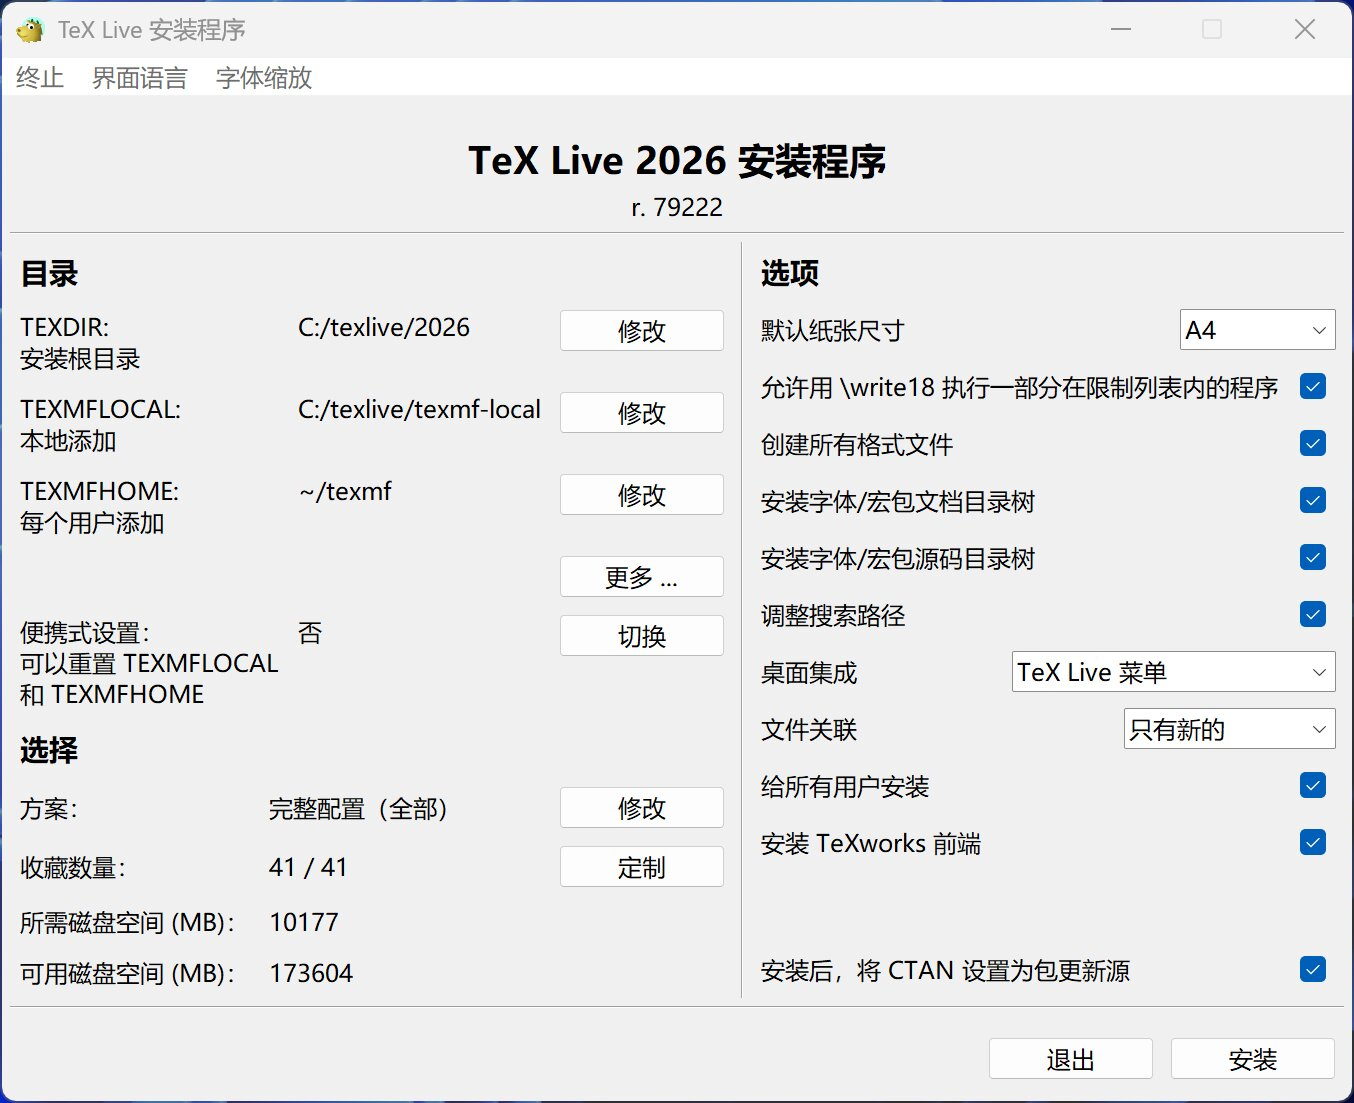
\includegraphics[width=1.0\linewidth]{win-texlive.jpg}
            \end{Figure}
        \end{column}
    \end{columns}
\end{frame}

\begin{frame}
    \frametitle{软件安装}
    Linux上，安装\LaTeX 这样庞大的软件只需要一句话
    \begin{Code}*
        \lstinputlisting{code/intro/apt-install.sh}
    \end{Code}
    这里\code{apt}是Ubuntu的\alert{软件包管理器}，它有三个关键特征
    \begin{itemize}
        \item 软件包集中化管理：软件集中在官方的软件仓库，不必去浏览器搜索。
        \item 软件安装方式统一：软件统一用\code{apt install}安装，自动解析依赖。
        \item 软件安装路径固定：在Linux上，软件安装的路径是有一套严格规范的。例如，执行程序会安装到\code{/bin}，库文件会安装到\code{/lib}，配置文件会安装到\code{/etc}，无需也不能手动选择。
    \end{itemize}
\end{frame}

\begin{frame}
    \frametitle{系统更新}
    \begin{columns}
        \begin{column}{0.53\textwidth}\setlength{\parskip}{6pt}
            Windows的系统更新常常让人感到恼火
            \begin{itemize}
                \item 强制推送：更新可能在工作一半时突然发生。
                \item 需要重启：更新意味着重启，不可热更新。
                \item 不透明性：更新改动时常会破坏系统。
                \item 体验割裂：更新只覆盖操作系统和预装应用。
            \end{itemize}
        \end{column}
        \begin{column}{0.45\textwidth}
            \begin{Figure}*
                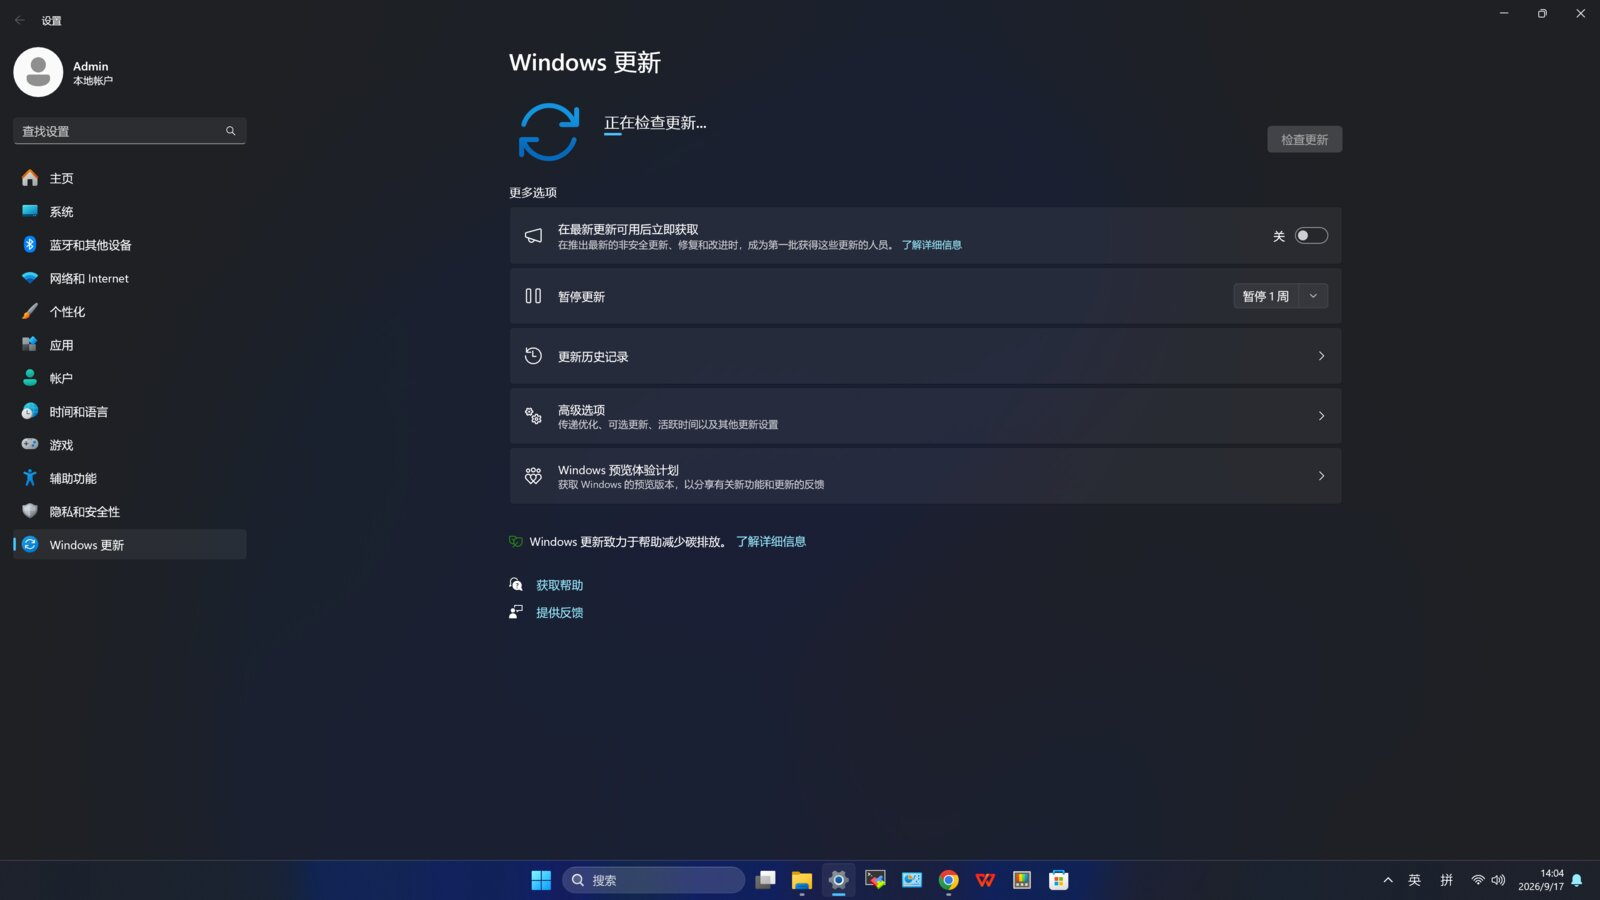
\includegraphics[width=1.0\linewidth]{win-update.jpg}
            \end{Figure}
        \end{column}
    \end{columns}
\end{frame}

\begin{frame}
    \frametitle{系统更新}
    Linux并不区分“系统软件”与“应用软件”，它们由同一个包管理器统一管理，可以一起更新
    \begin{Code}*
        \lstinputlisting{code/intro/apt-upgrade.sh}
    \end{Code}
    其中，\code{apt update}用于刷新软件包索引，\code{apt upgrade}用于下载并安装更新。

    你可以随时执行这两条命令，更新完成后\alert{无需重启}！
\end{frame}

\begin{frame}
    \frametitle{路径与命令}
    Windows在路径与命令的设计上自成一派，与几乎所有其他操作系统都不同
    \begin{itemize}
        \item 路径用反斜杠\texttt{\textbackslash{}}而非正斜杠\code{/}分隔，且从盘符\code{C:}或\code{D:}开始，没有统一的根目录。
        \item 路径的反斜杠\texttt{\textbackslash{}}是大多数编程语言中的转义符，表示\texttt{\textbackslash{}}本身要用\texttt{\textbackslash{}\textbackslash{}}转义。于是经常需要将\texttt{C:\textbackslash{}Users\textbackslash{}liyuxuan}这样的路径写成\texttt{C:\textbackslash{}\textbackslash{}Users\textbackslash{}\textbackslash{}liyuxuan}，既别扭又容易出错。
        \item 系统目录组织混乱，且存在\texttt{C:\textbackslash{}Program Files}和\texttt{C:\textbackslash{}Program Files (x86)}这种极为糟糕的关键系统目录名称选择：路径中的空格和括号是灾难！命令行中对此需要特殊处理。
        \item Windows的命令行\code{cmd}非常难用，命令名称和选项格式与主流操作系统格格不入：无法使用\code{cd}、\code{ls}、\code{mkdir}、\code{cp}、\code{rm}等常用命令，使用\code{/}而非\code{-}或\code{--}表示选项（例如\code{dir /a}）。
    \end{itemize}
\end{frame}

\begin{frame}
    \frametitle{POSIX：类Unix系统的共同规范}
    \begin{vspquote}{Windows才是那个异类}
        Windows的这些特性并非来自深思熟虑的工程设计，而是一次次历史妥协的结果。
        
        Windows虽然是全球最流行的桌面操作系统，但它才是那个异类！
    \end{vspquote}
    Windows之外的几乎所有操作系统（包括Linux的各个发行版和MacOS）都遵循了一套统一的接口标准——\alert{POSIX}（Portable Operating System Interface），它规定了命令、路径、进程、文件等应当如何工作。POSIX是所有类Unix系统共同遵循的规范，具体来说，它意味着
    \begin{itemize}
        \item 存在统一的\code{/}根目录，使用正斜杠\code{/}作为路径分隔符（例如\code{/home/liyuxuan}）。
        \item 存在\code{/bin}、\code{/lib}、\code{/etc}等标准目录，这被称为\alert{FHS}（Filesystem Hierarchy Standard）。
        \item 存在\code{cd}、\code{ls}、\code{mkdir}、\code{cp}、\code{rm}等标准命令，\code{-}表示短选项（\code{-l}），\code{--}表示长选项（\code{--help}）。
    \end{itemize}
    Windows是主流操作系统中唯一与Unix没有继承关系、也不遵循POSIX的系统！
\end{frame}

\begin{frame}
    \frametitle{开发环境}
    \begin{vspquote}{Windows是编程学习的最大阻碍}
        Windows糟糕的命令行体验使得许多教程无法使用：我该在哪里敲这个命令？
    \end{vspquote}
    Windows上编程，往往要先请出一个庞大的\alert{IDE}（Integrated Development Environment）
    \begin{itemize}
        \item 开发C/C++通常要安装体积巨大的Visual Studio，其使用专有的MSVC编译器。
        \item 开发Python通常要安装Anaconda，其核心的环境管理功能被臃肿的GUI界面层层包裹。
        \item 把“编译、运行”包装在层层按钮之后，容易让人困在表象，忽略背后真正发生了什么。
        \item 当真的需要敲命令时，又要面对糟糕的\code{cmd}，甚至不知道命令该在哪里输入。
    \end{itemize}
\end{frame}

\begin{frame}
    \frametitle{开发环境}
    Linux上，C编译器和Python解释器都是很常规的命令行工具，很容易使用
    \begin{Code}*
        \lstinputlisting{code/intro/dev.sh}
    \end{Code}
    至于你在哪里编写\code{main.c}和\code{main.py}？这是编辑器的工作，你可以使用最流行的VSCode或历史悠久的Vim，但这不重要：用什么编写代码和用什么运行代码，是毫无关系的两件事。

    每个工具只做好一件事，再通过命令行组合起来，这正是Unix哲学。
\end{frame}

\begin{frame}
    \frametitle{Linux不只是命令行}
    Linux是一个成熟的桌面操作系统：它有完善的图形界面，日常使用与任何系统无异！
    \begin{itemize}
        \item 你可以用鼠标点击连接蓝牙和无线网络（我并不知道通过命令行怎么做）。
        \item 在\code{cd}和\code{ls}之外，Ubuntu也有图形化的文件浏览器Nautilus（文件）。
        \item 在\code{apt}之外，Ubuntu也有图形化的软件商店Synaptic（新立得）。
        \item 高效的命令行是Linux强大的一面，但不代表一切事情都需要通过命令行完成。
    \end{itemize}
\end{frame}

\begin{frame}
    \frametitle{Linux不只是命令行}
    \begin{columns}
        \begin{column}{0.48\textwidth}
            \begin{Figure}*[Nautilus]
                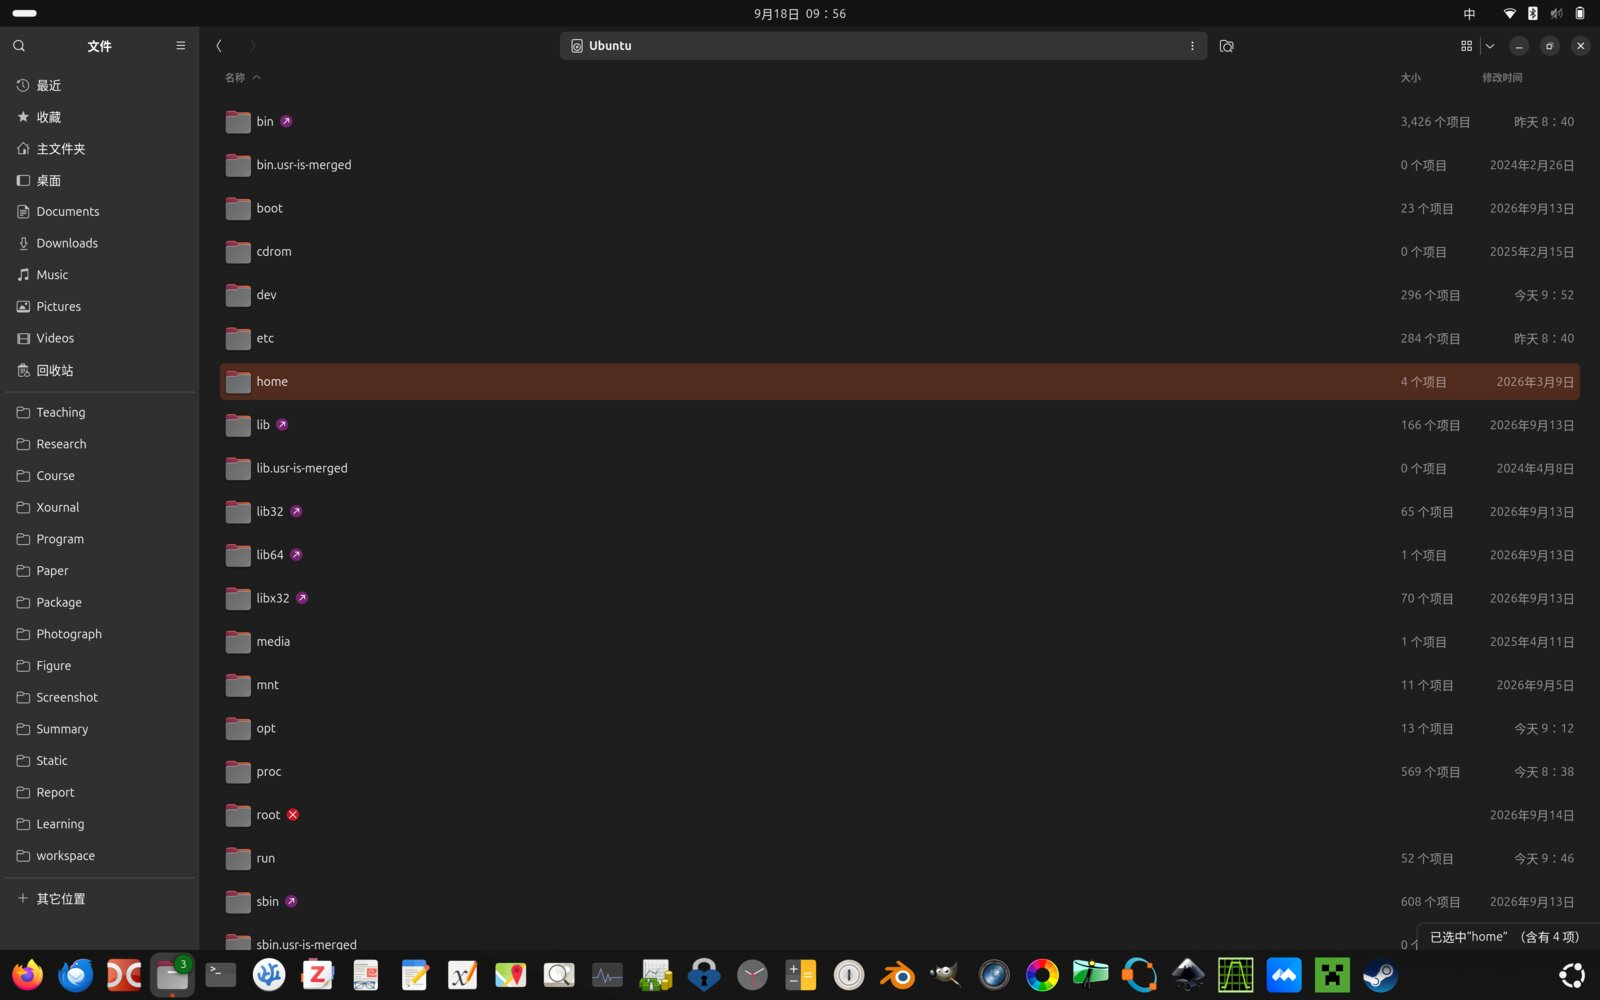
\includegraphics[width=\linewidth]{screen-nautilus.jpg}  
            \end{Figure}
        \end{column}
        \begin{column}{0.48\textwidth}
            \begin{Figure}*[Synaptic]
                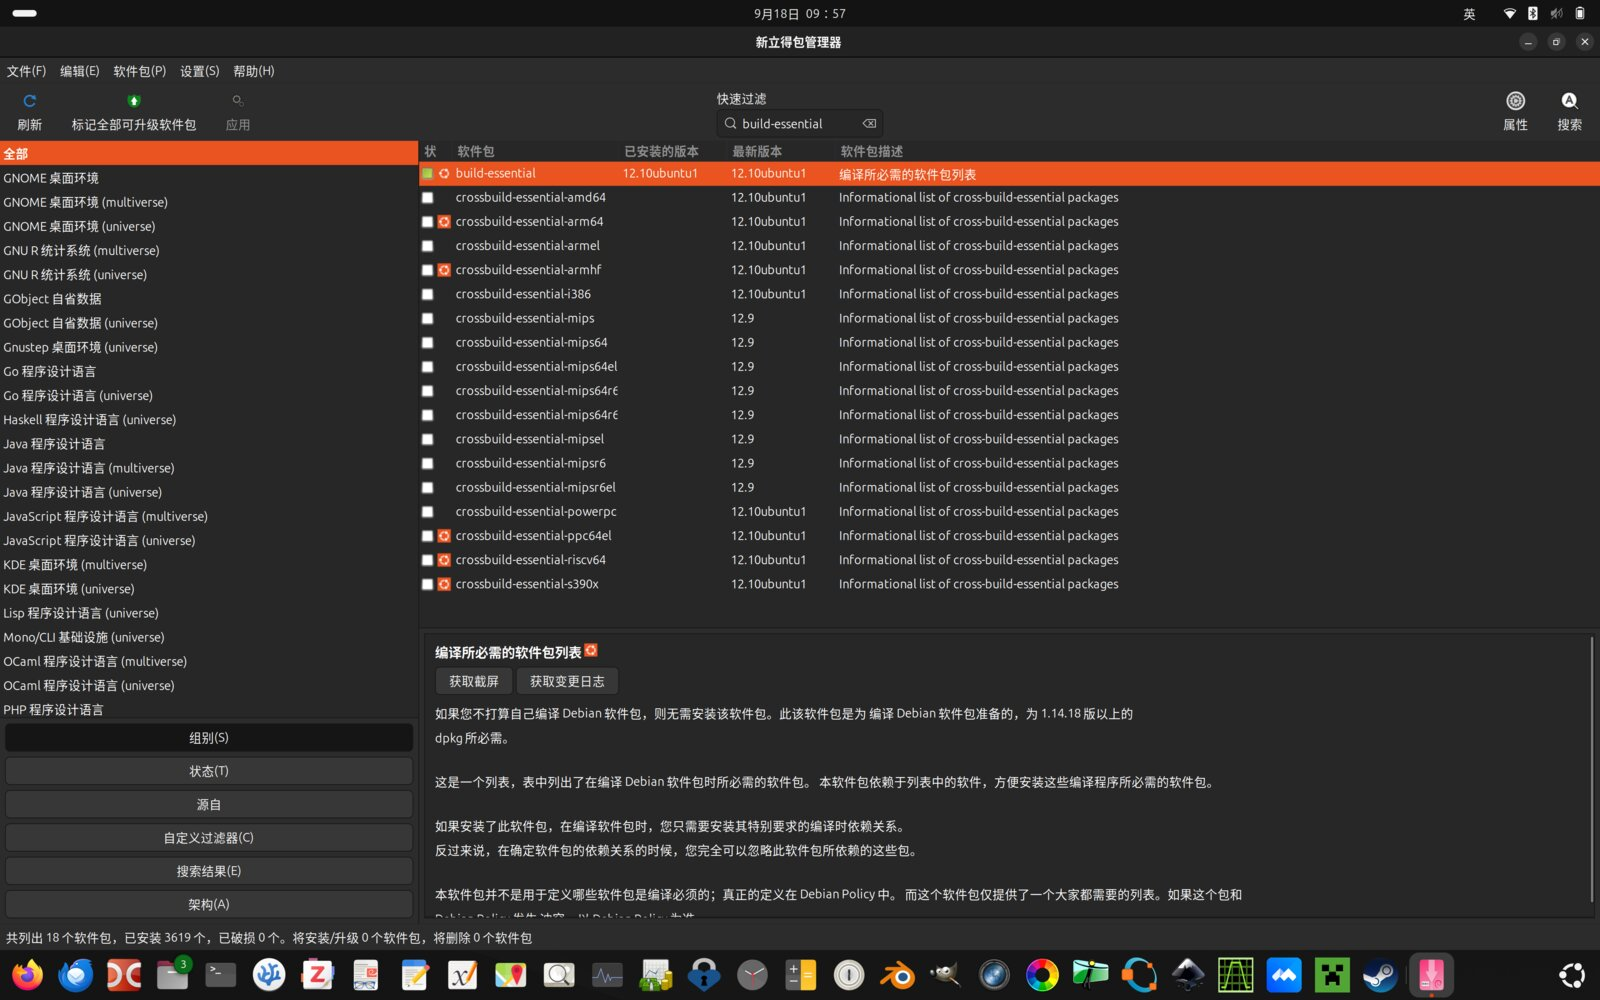
\includegraphics[width=\linewidth]{screen-synaptic.jpg}  
            \end{Figure}
        \end{column}
    \end{columns}
\end{frame}

\begin{frame}
    \frametitle{Linux也有丰富的软件生态}
    Linux常常被质疑的另外一点是软件生态：我需要使用的软件会不会没有Linux支持？
    \begin{itemize}
        \item 有些商业软件实际上有非常全面的Linux支持，商业软件和开源系统并不矛盾。
        \item 有些商业软件实际上有功能相当甚至更好的开源软件替代！
        \item 当然，我们需要承认，确实有一部分软件只提供了Windows支持。
    \end{itemize}
\end{frame}

\begin{frame}
    \frametitle{文档与表格}
    \begin{itemize}
        \item 图形化编辑文档本身，其实就是一件糟糕的事。
        \item Word：Markdown或LaTeX写作是更好的选择，内容与格式分离，纯文本便于版本管理。
        \item PowerPoint：Markdown有Marp，LaTeX有Beamer，幻灯片本质只是一种特殊的文档。
        \item Excel：表格数据可以用\code{.csv}存储，表格分析可以用\code{pandas}等Python库处理。
        \item 当然，如果仍然需要传统Office软件，开源的有LibreOffice可用，商业的有WPS可用。
        \item PDF阅读器通常是系统预装的，Ubuntu会搭配Evince（文档查看器）。
    \end{itemize}
\end{frame}

\begin{frame}
    \frametitle{文档与表格}
    \begin{columns}
        \begin{column}{0.48\textwidth}
            \begin{Figure}*[Markdown]
                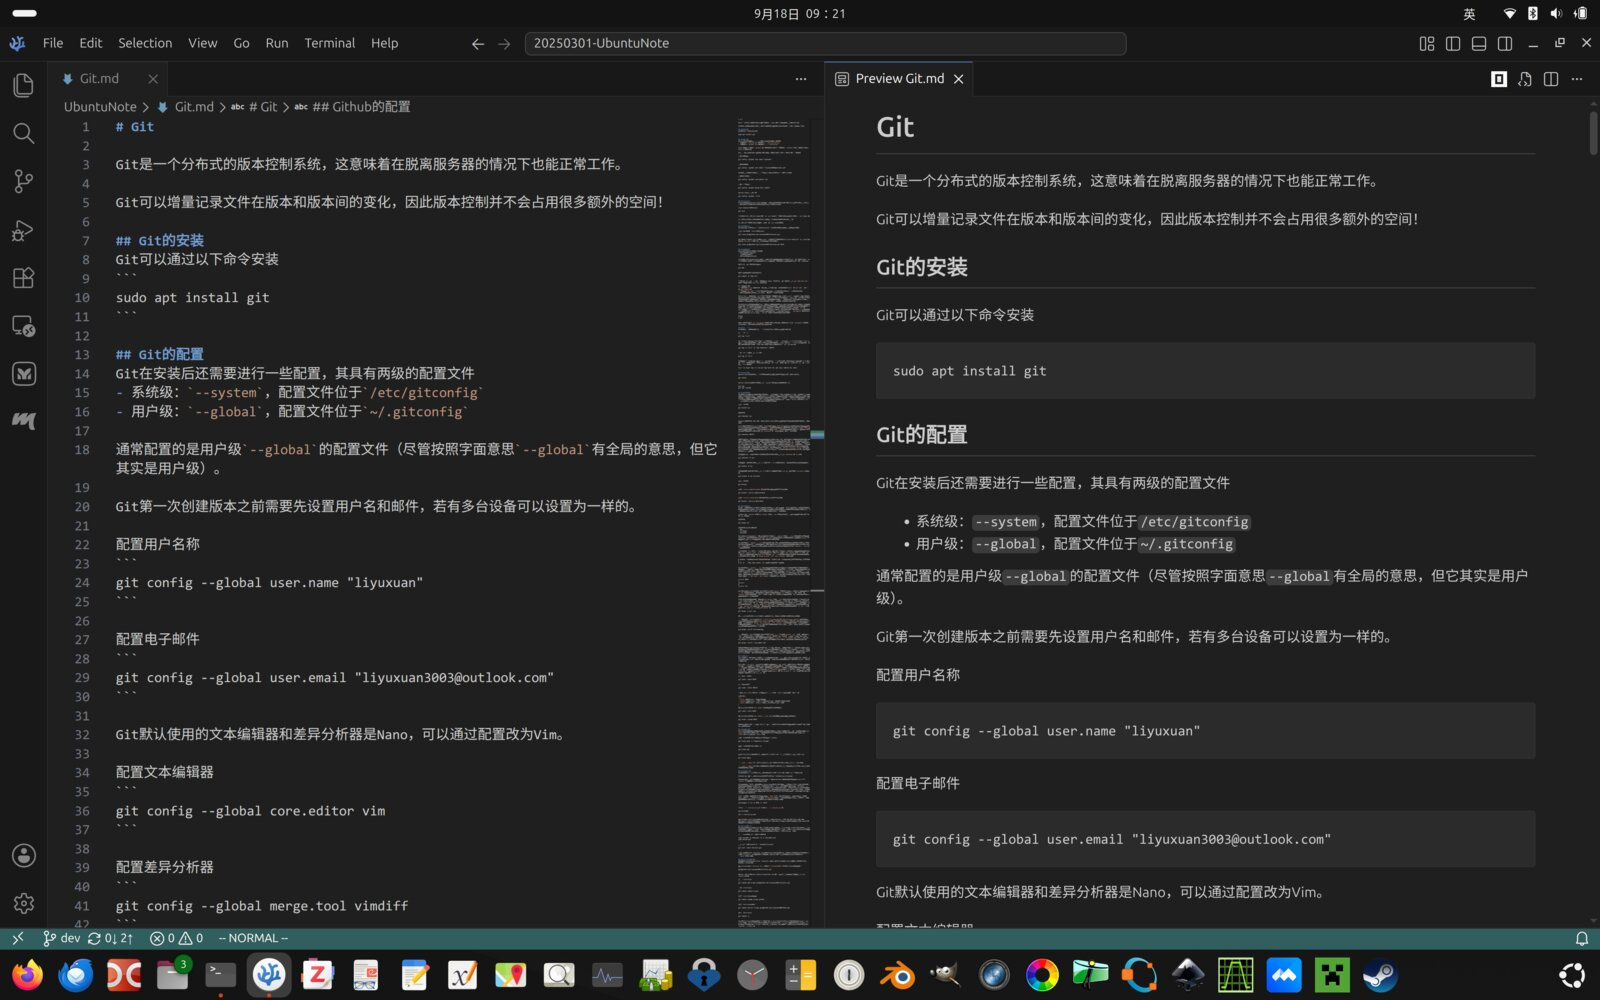
\includegraphics[width=\linewidth]{screen-markdown.jpg}  
            \end{Figure}
        \end{column}
        \begin{column}{0.48\textwidth}
            \begin{Figure}*[LaTeX]
                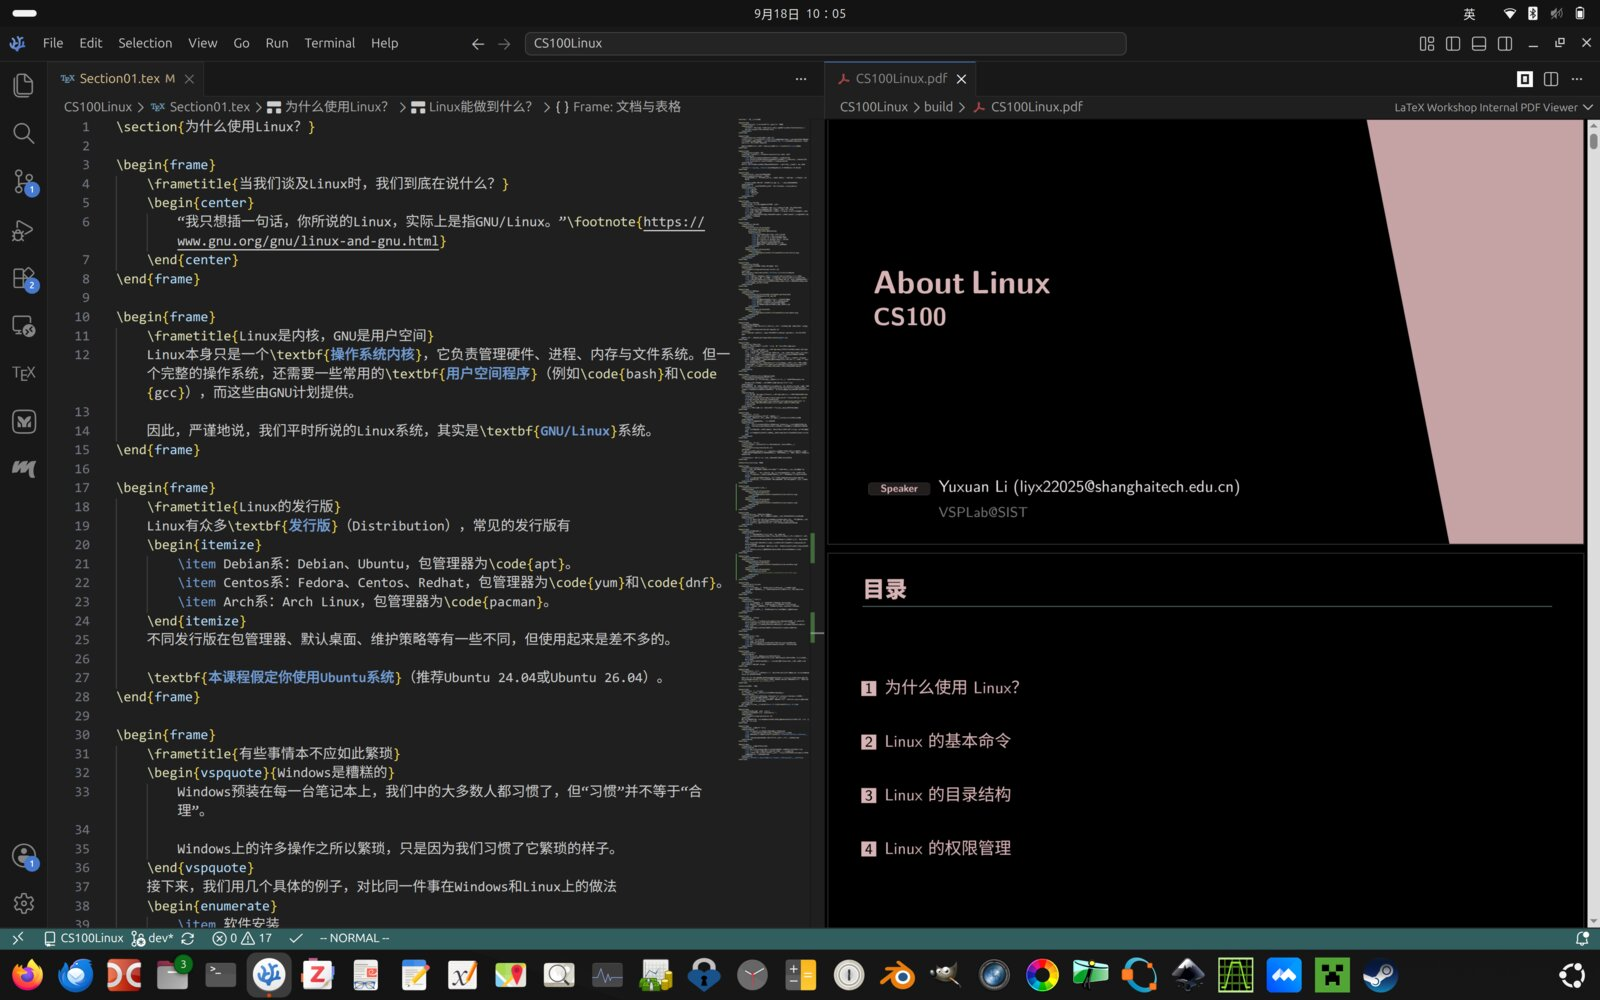
\includegraphics[width=\linewidth]{screen-latex.jpg}  
            \end{Figure}
        \end{column}
    \end{columns}
\end{frame}

\begin{frame}
    \frametitle{网络与通信}
    \begin{itemize}
        \item 浏览器可以使用开源的Firefox，当然Chrome也是同样可用的。
        \item 邮件客户端可以使用开源的Thunderbird，它的体验远好于现在的Outlook (New)。
    \end{itemize}
\end{frame}

\begin{frame}
    \frametitle{网络与通信}
    \begin{columns}
        \begin{column}{0.48\textwidth}
            \begin{Figure}*[Firefox]
                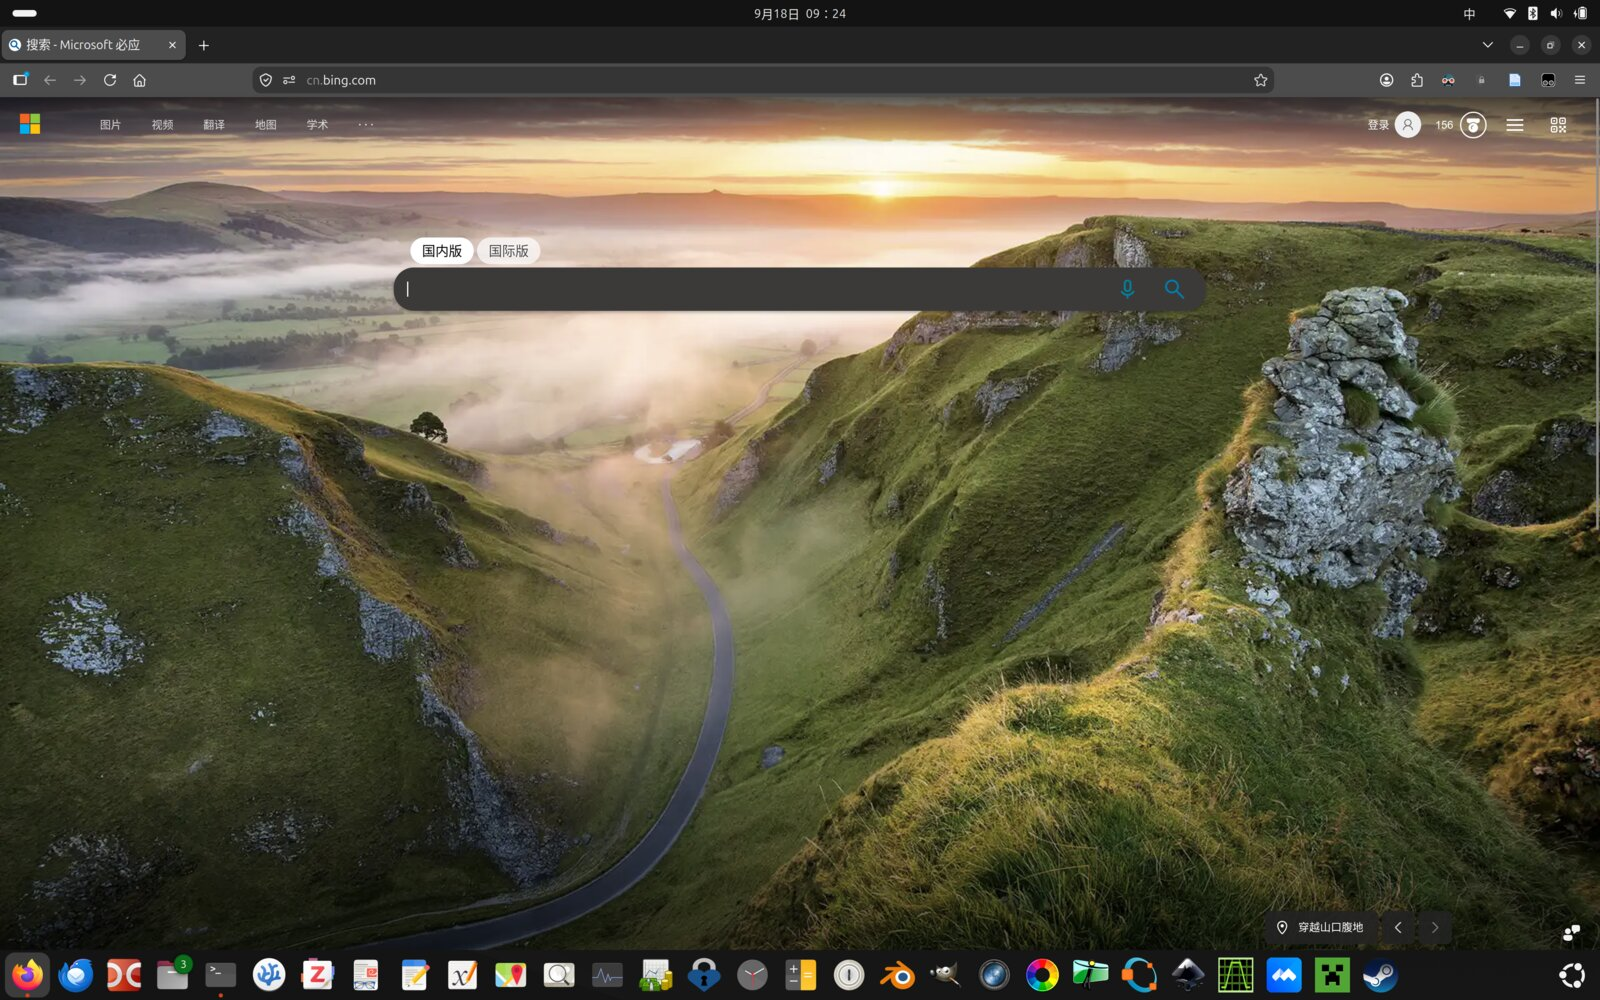
\includegraphics[width=\linewidth]{screen-firefox.jpg}  
            \end{Figure}
        \end{column}
        \begin{column}{0.48\textwidth}
            \begin{Figure}*[Thunderbird]
                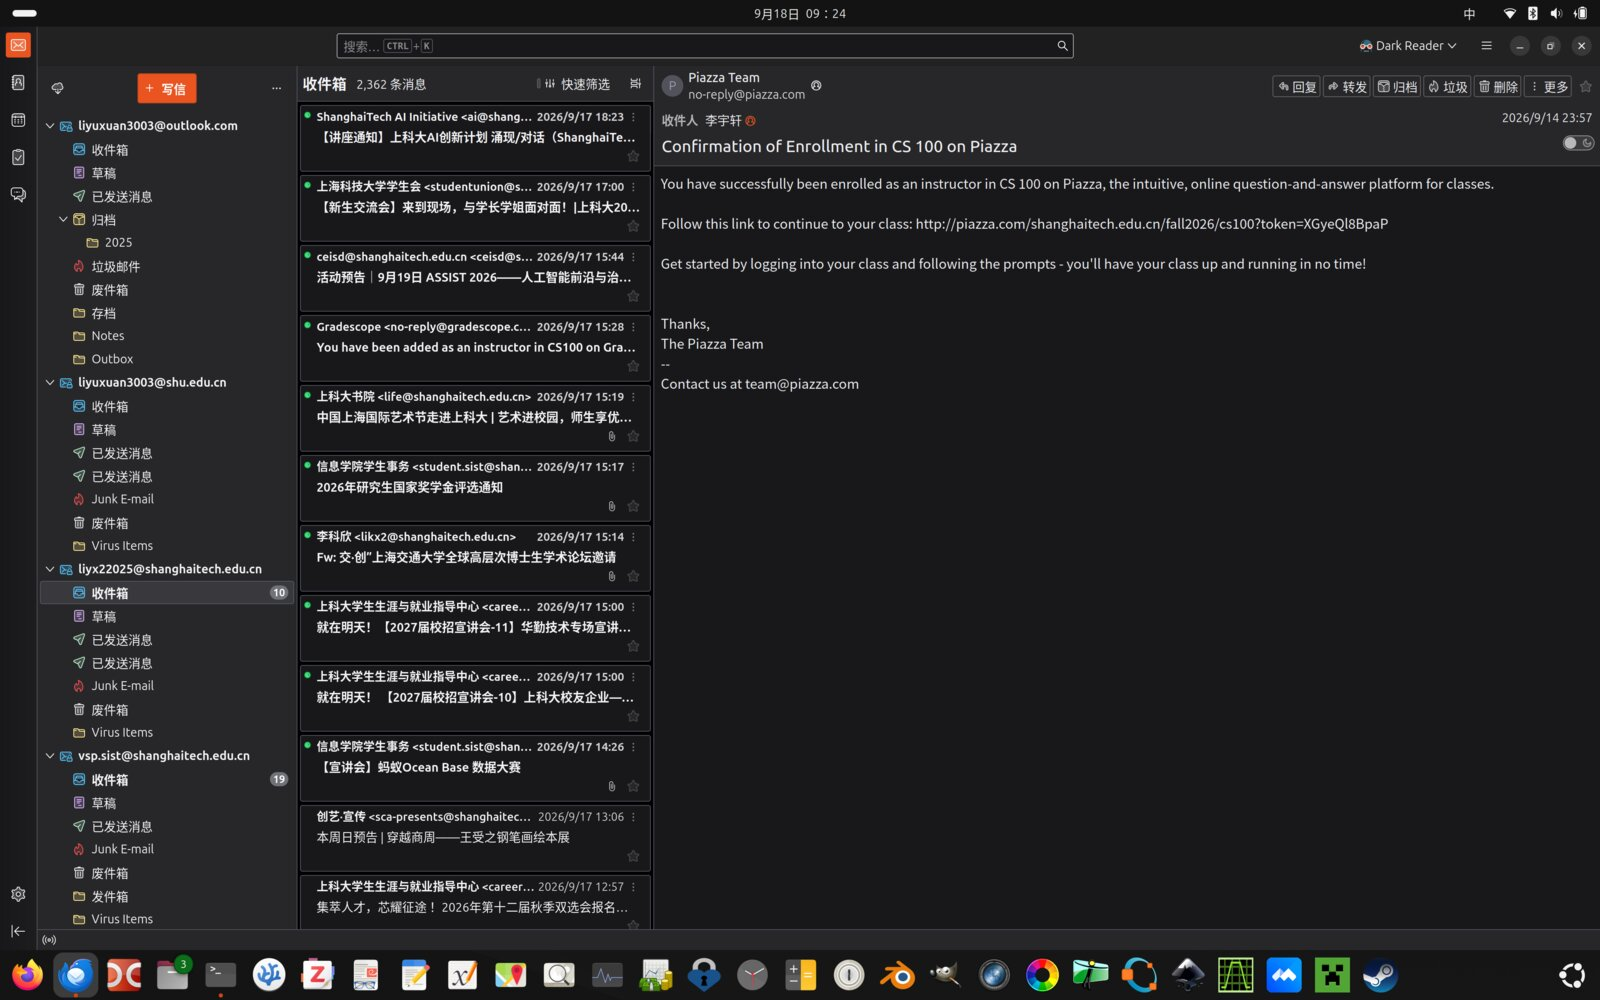
\includegraphics[width=\linewidth]{screen-thunderbird.jpg}  
            \end{Figure}
        \end{column}
    \end{columns}
\end{frame}

\begin{frame}
    \frametitle{图形与影像}
    \begin{itemize}
        \item 位图处理：可以使用开源的GIMP，替代Adobe Photoshop。
        \item 矢量绘图：可以使用开源的Inkscape，替代Adobe Illustrator。
        \item 照片处理：可以使用开源的RawTherapee和Digikam，替代Adobe Lightroom。
        \item 三维创作：可以使用开源的Blender，它是该领域的主力生产工具！
    \end{itemize}
\end{frame}

\begin{frame}
    \frametitle{图形与影像}
    \begin{columns}
        \begin{column}{0.48\textwidth}
            \begin{Figure}*[Inkscape]
                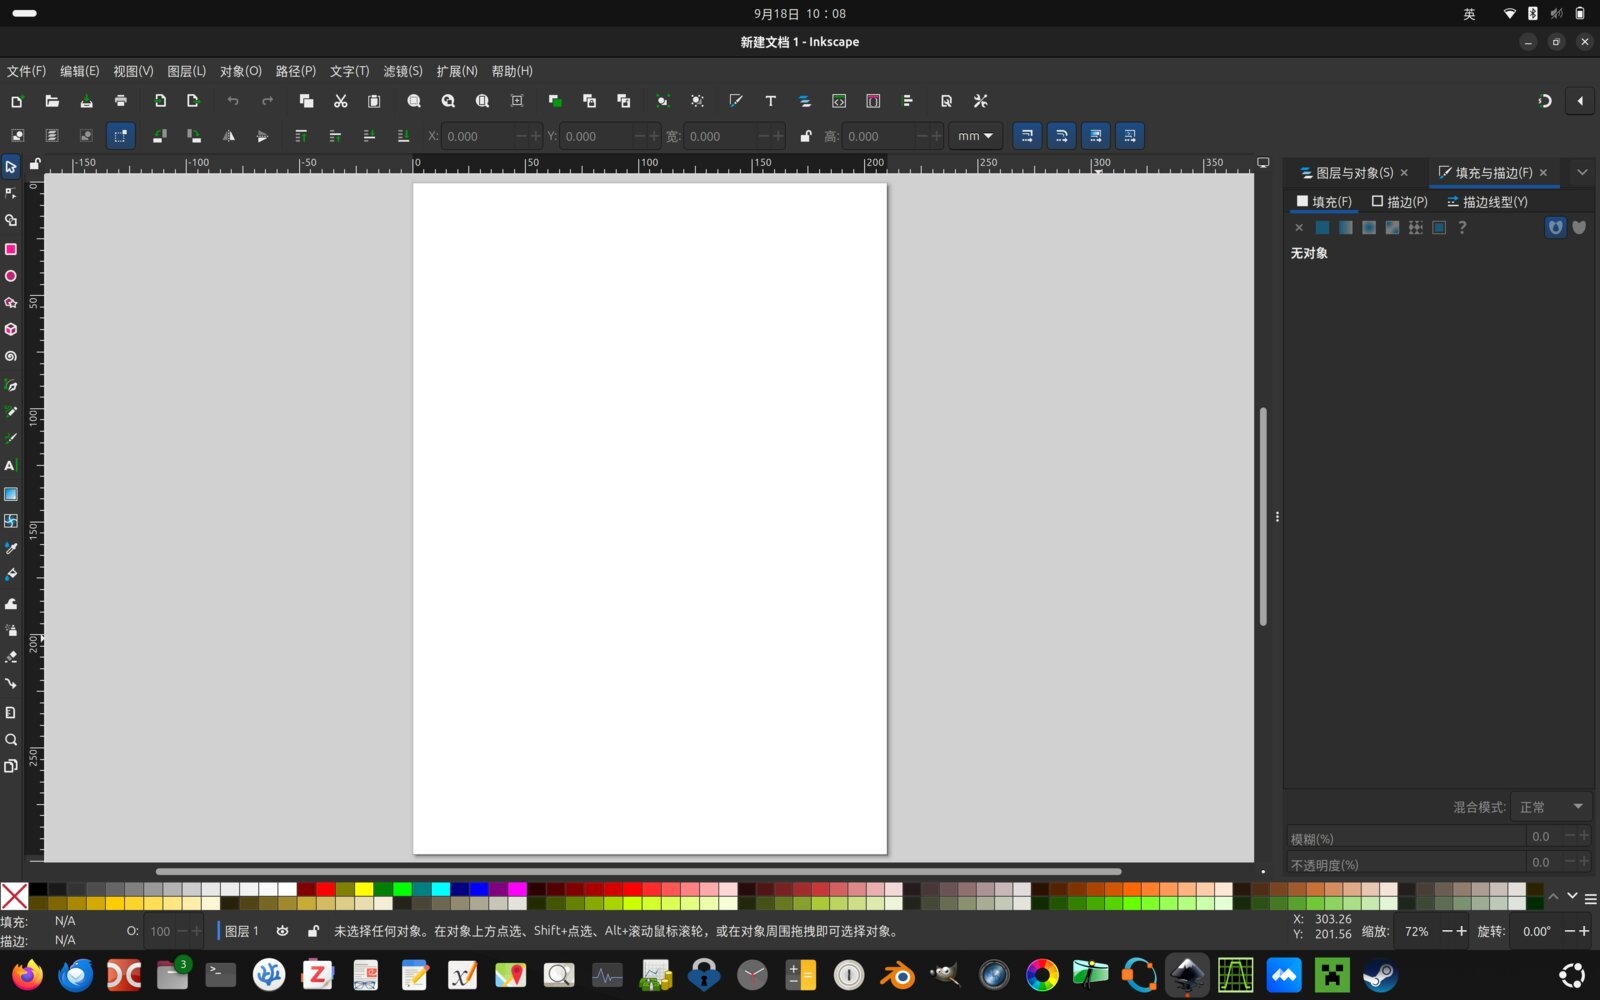
\includegraphics[width=\linewidth]{screen-inkscape.jpg}  
            \end{Figure}
        \end{column}
        \begin{column}{0.48\textwidth}
            \begin{Figure}*[Blender]
                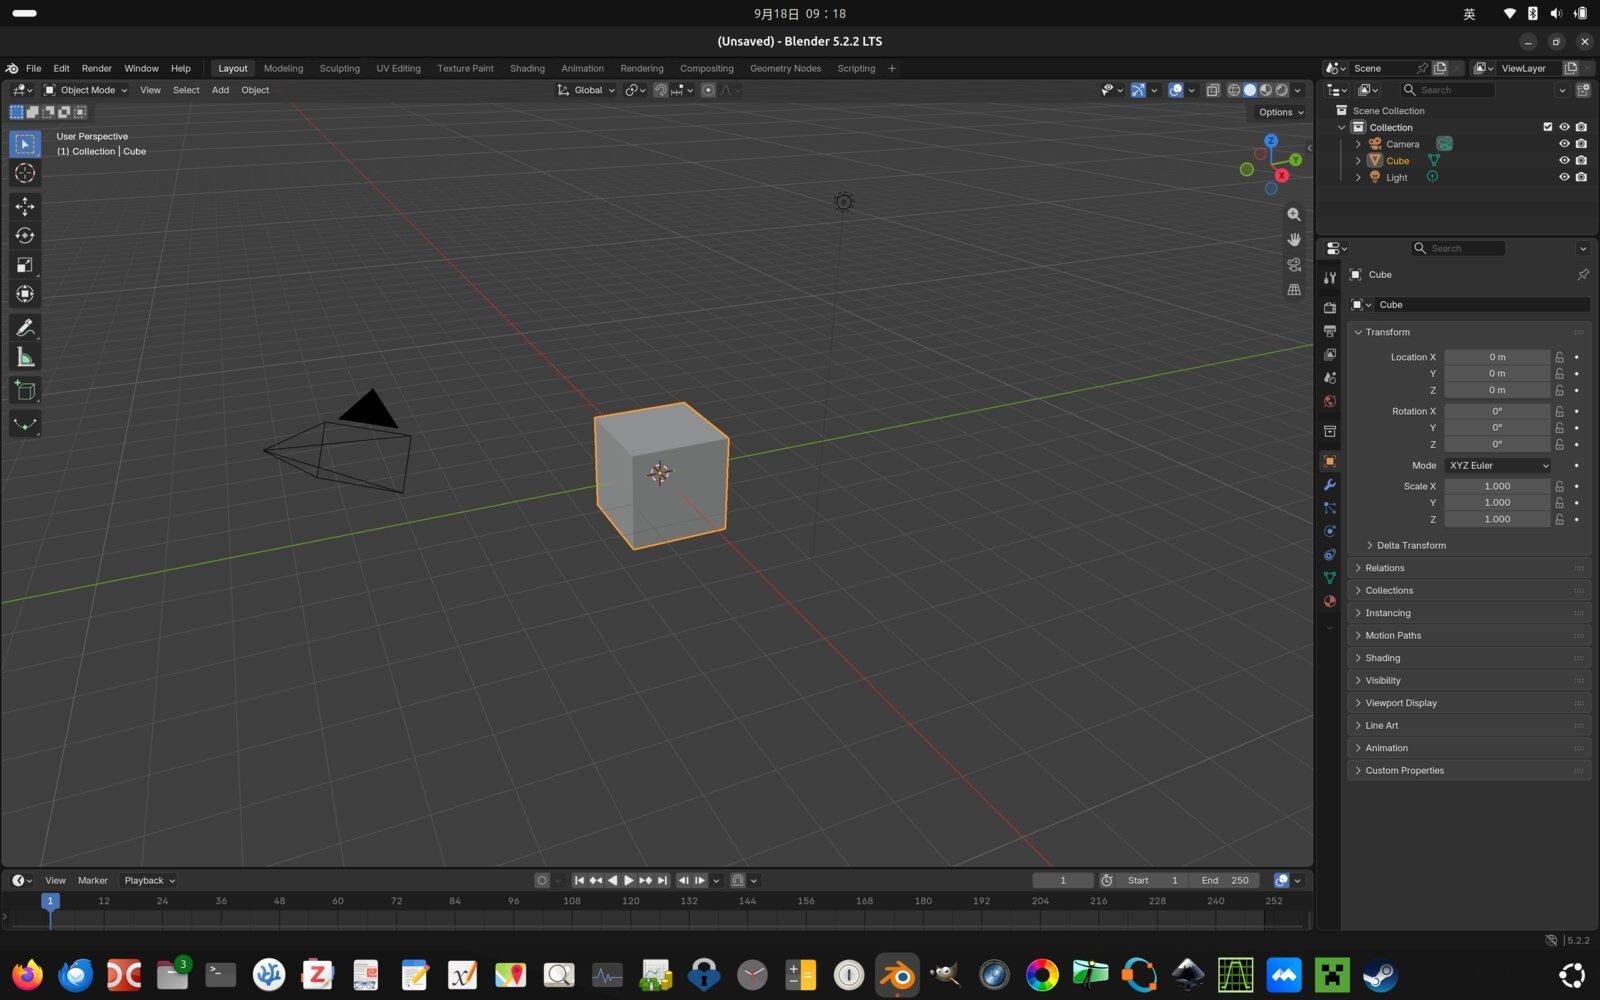
\includegraphics[width=\linewidth]{screen-blender.jpg}  
            \end{Figure}
        \end{column}
    \end{columns}
\end{frame}

\begin{frame}
    \frametitle{开发工具}
    \begin{itemize}
        \item C/C++开发：直接使用\code{gcc}、\code{g++}、\code{make}等命令。
        \item Python开发：直接使用\code{python}命令，配合\code{uv}、\code{conda}管理虚拟环境。
        \item ARM嵌入式开发不必依赖Keil，可以使用\code{gcc-arm-none-eabi}的开源工具链替代。
        \item 代码编辑器：VSCode同样可用，VSCodium则是更为纯净的开源构建版本。
    \end{itemize}
\end{frame}

\begin{frame}
    \frametitle{开发工具}
    \begin{columns}
        \begin{column}{0.48\textwidth}
            \begin{Figure}*[C++]
                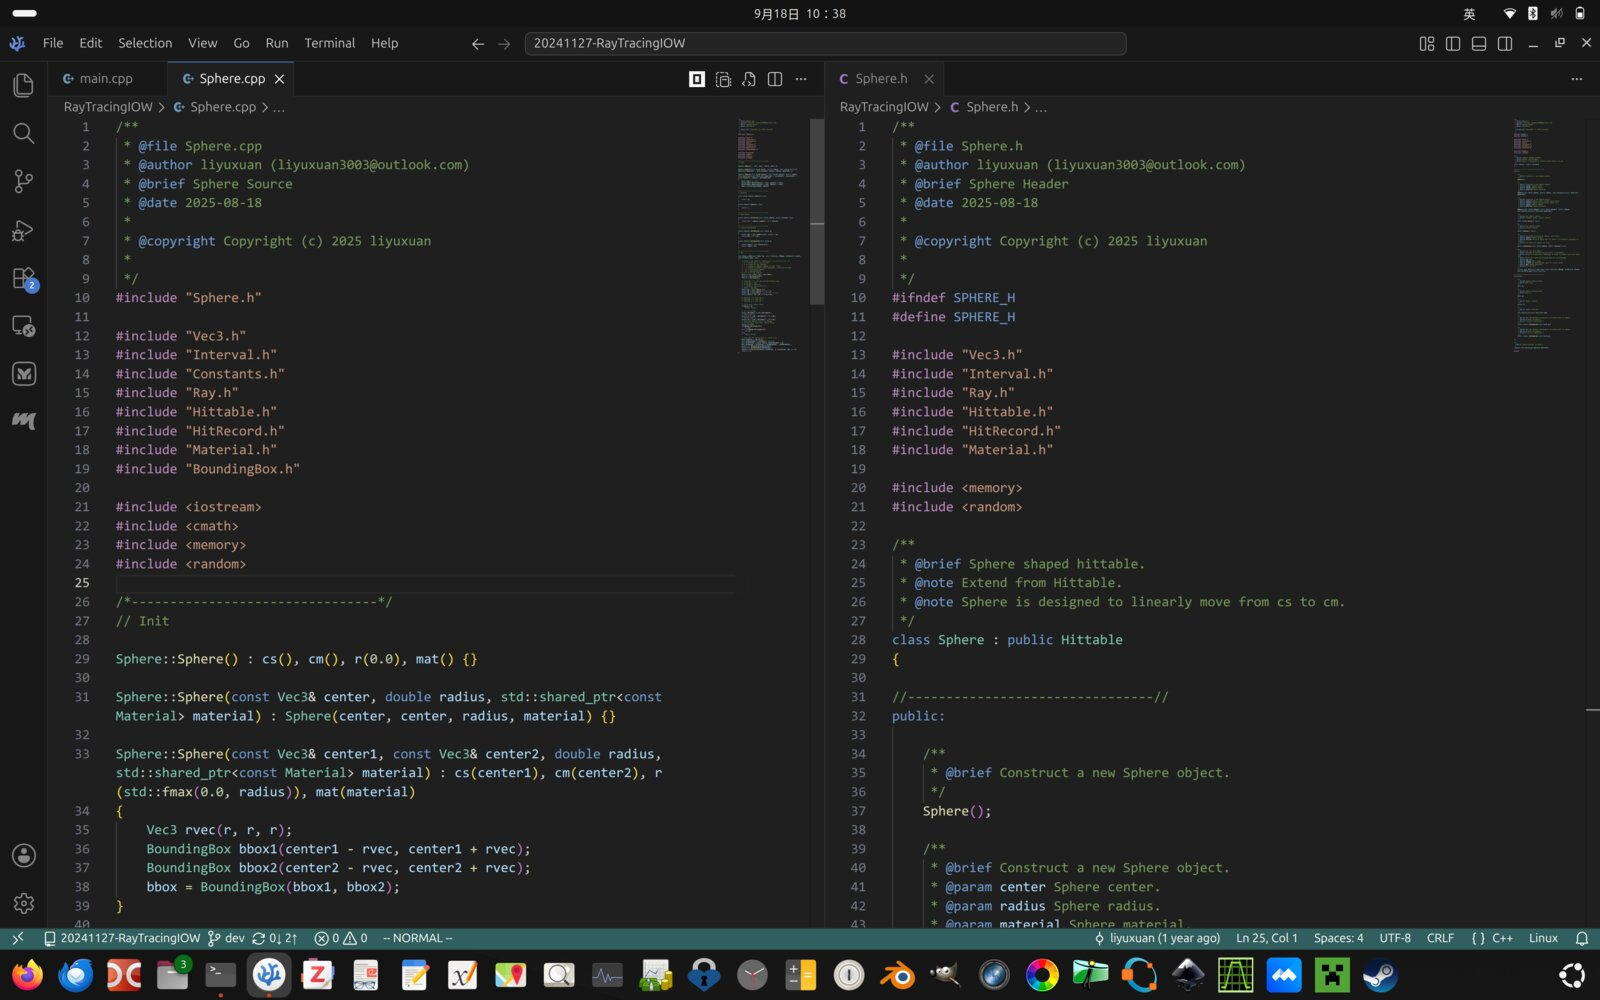
\includegraphics[width=\linewidth]{screen-cpp.jpg}  
            \end{Figure}
        \end{column}
        \begin{column}{0.48\textwidth}
            \begin{Figure}*[Python]
                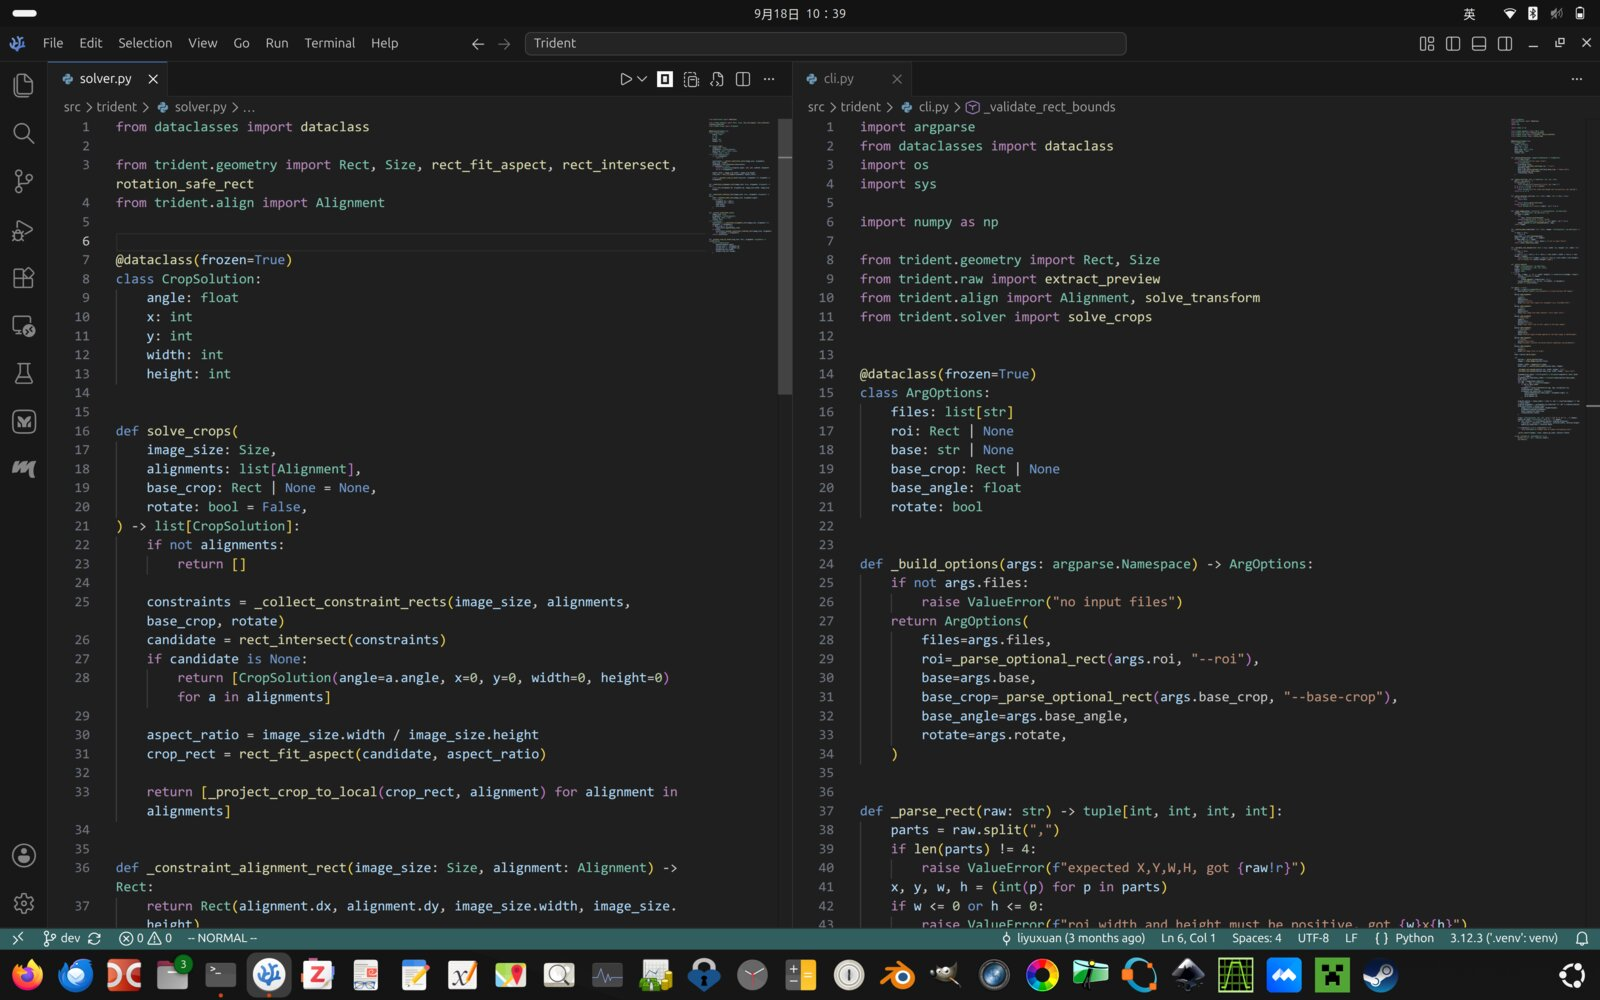
\includegraphics[width=\linewidth]{screen-python.jpg}  
            \end{Figure}
        \end{column}
    \end{columns}
\end{frame}

\begin{frame}
    \frametitle{工程软件}
    \begin{itemize}
        \item 电路设计：使用开源的KiCad（立创EDA也是基于KiCad！），替代Altium等商业应用。
        \item 机械设计：使用开源的FreeCad，替代Inventor和SolidWorks等商业应用。
        \item FPGA：Vivado提供Linux版本，仿真可以使用开源的Verilator与GTKWave。
        \item 符号计算：Mathematica提供Linux版本。
        \item 数值计算：Matlab提供Linux版本，也有命令兼容的开源替代Octave可用。
    \end{itemize}
\end{frame}

\begin{frame}
    \frametitle{工程软件}
    \begin{columns}
        \begin{column}{0.48\textwidth}
            \begin{Figure}*[KiCad]
                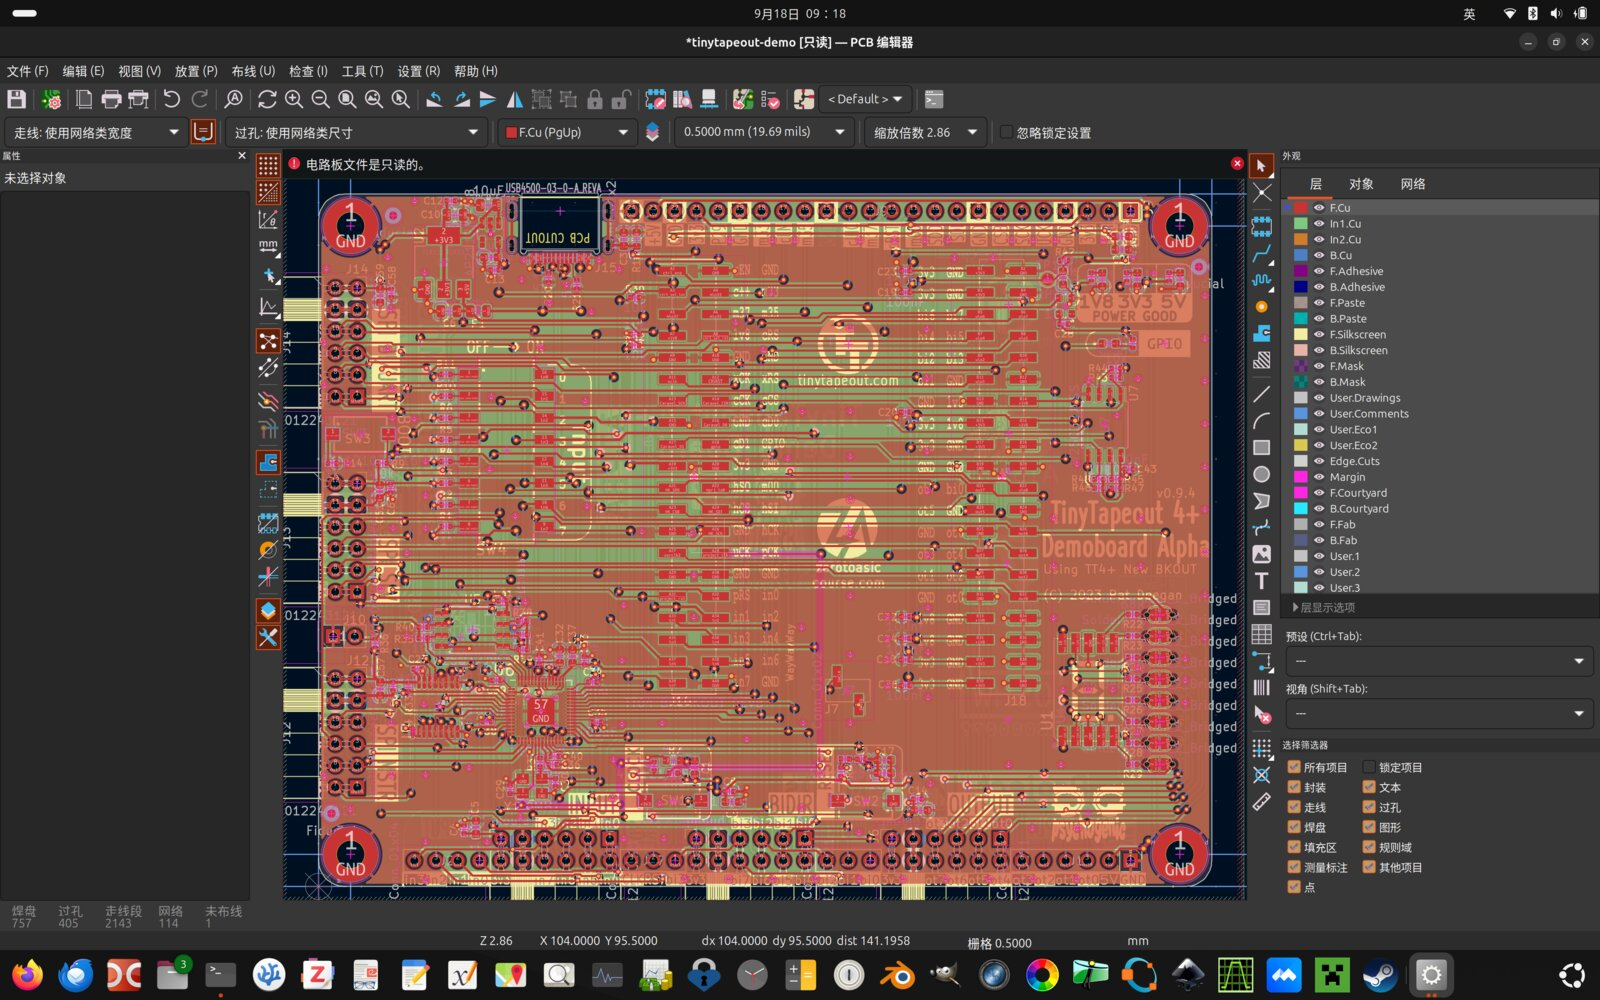
\includegraphics[width=\linewidth]{screen-kicad.jpg}  
            \end{Figure}
        \end{column}
        \begin{column}{0.48\textwidth}
            \begin{Figure}*[FreeCAD]
                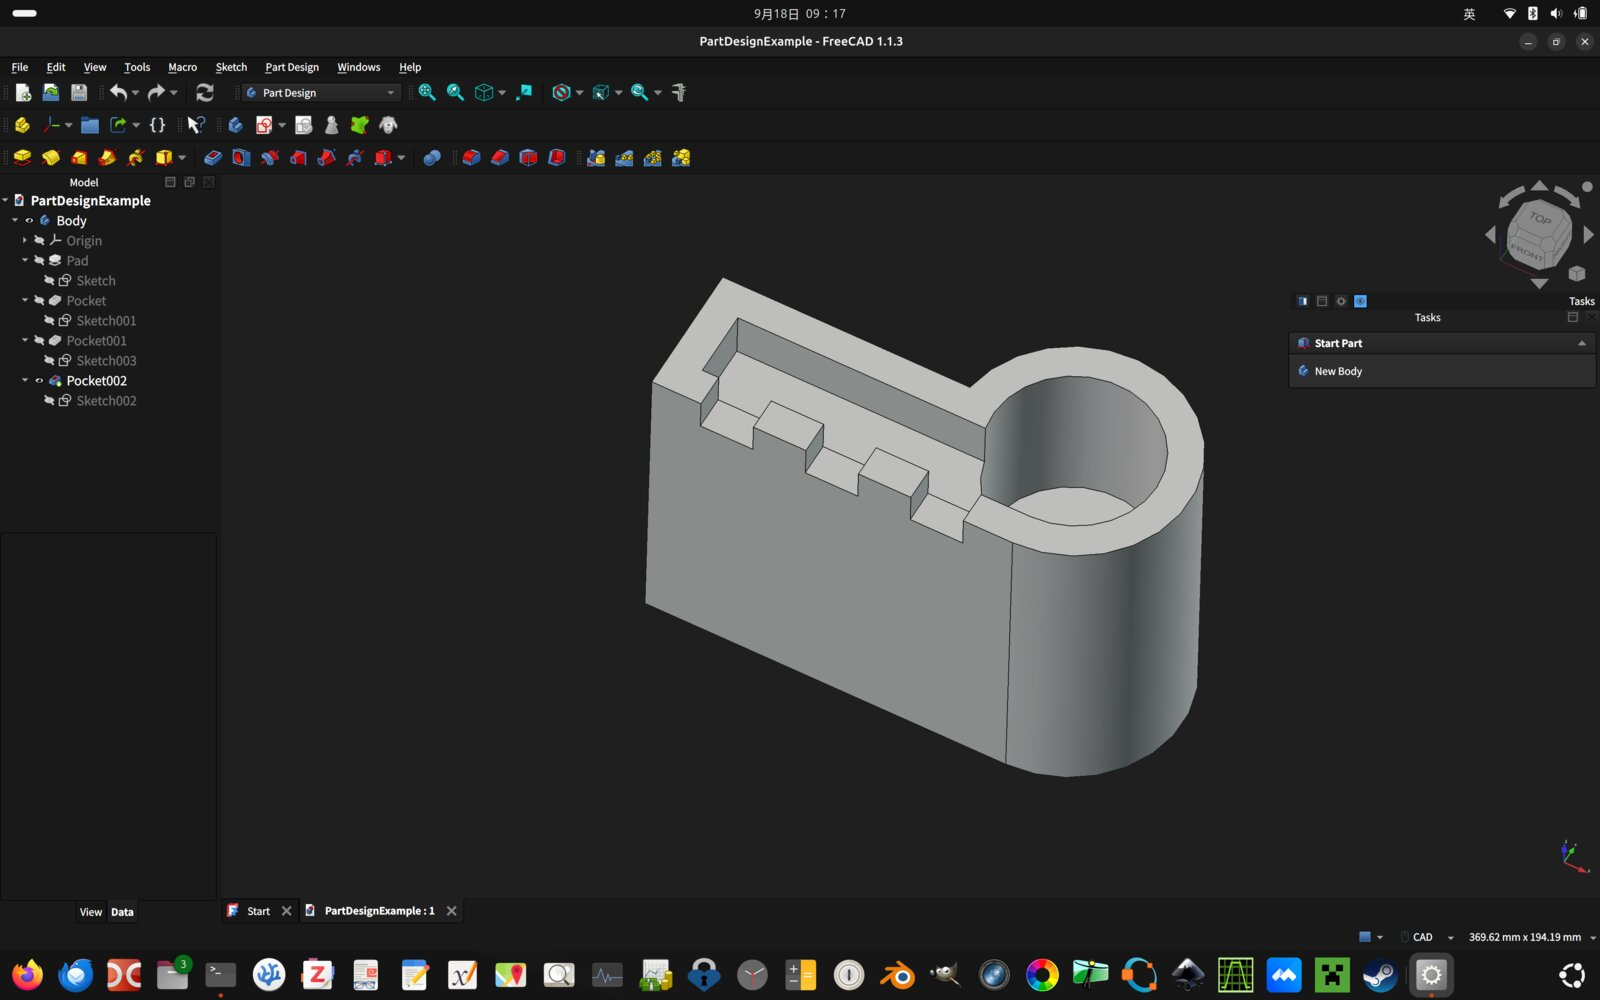
\includegraphics[width=\linewidth]{screen-freecad.jpg}  
            \end{Figure}
        \end{column}
    \end{columns}
\end{frame}

\begin{frame}
    \frametitle{游戏}
    \begin{itemize}
        \item 游戏常常被认为是Windows平台的专属，但其实Linux上也可以畅玩大部分游戏！
        \item Minecraft原生支持Linux系统，可以直接玩（仅Java版，不支持Bedrock版）。
        \item Steam提供了兼容层Proton，\alert{绝大多数Steam游戏都可以直接运行}！
        \item Steam OS自身就是一个基于Arch Linux修改的系统。
    \end{itemize}
\end{frame}

\begin{frame}
    \frametitle{游戏}
    \begin{columns}
        \begin{column}{0.48\textwidth}
            \begin{Figure}*[Minecraft]
                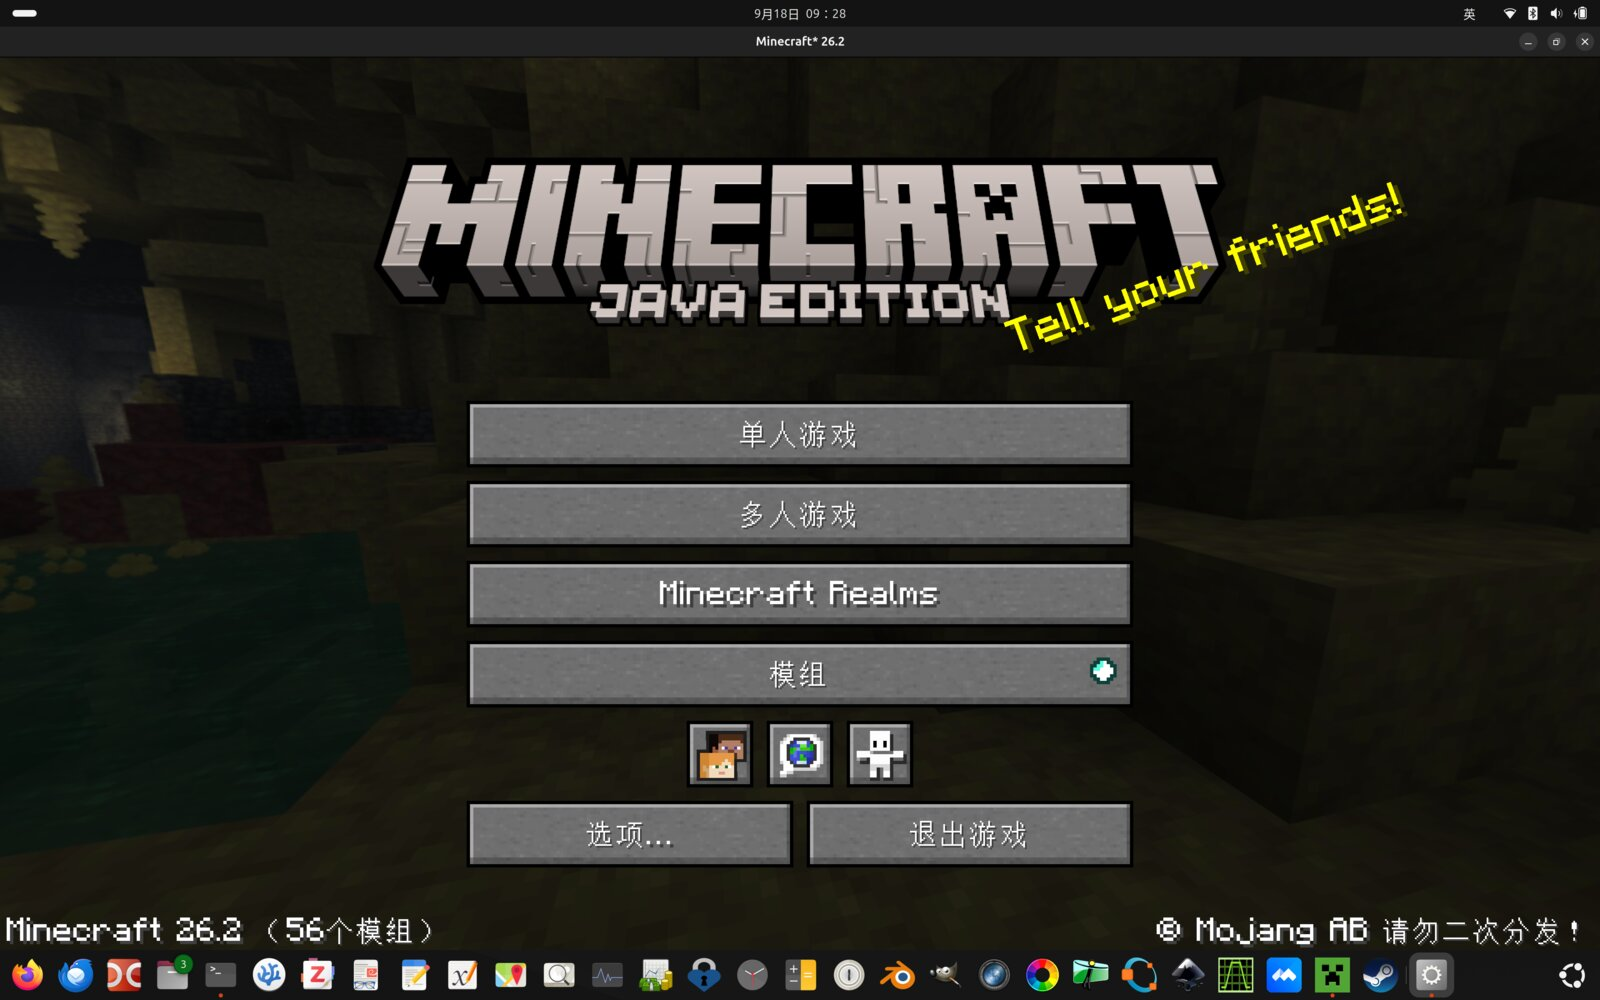
\includegraphics[width=\linewidth]{screen-minecraft.jpg}  
            \end{Figure}
        \end{column}
        \begin{column}{0.48\textwidth}
            \begin{Figure}*[Age of Empires II]
                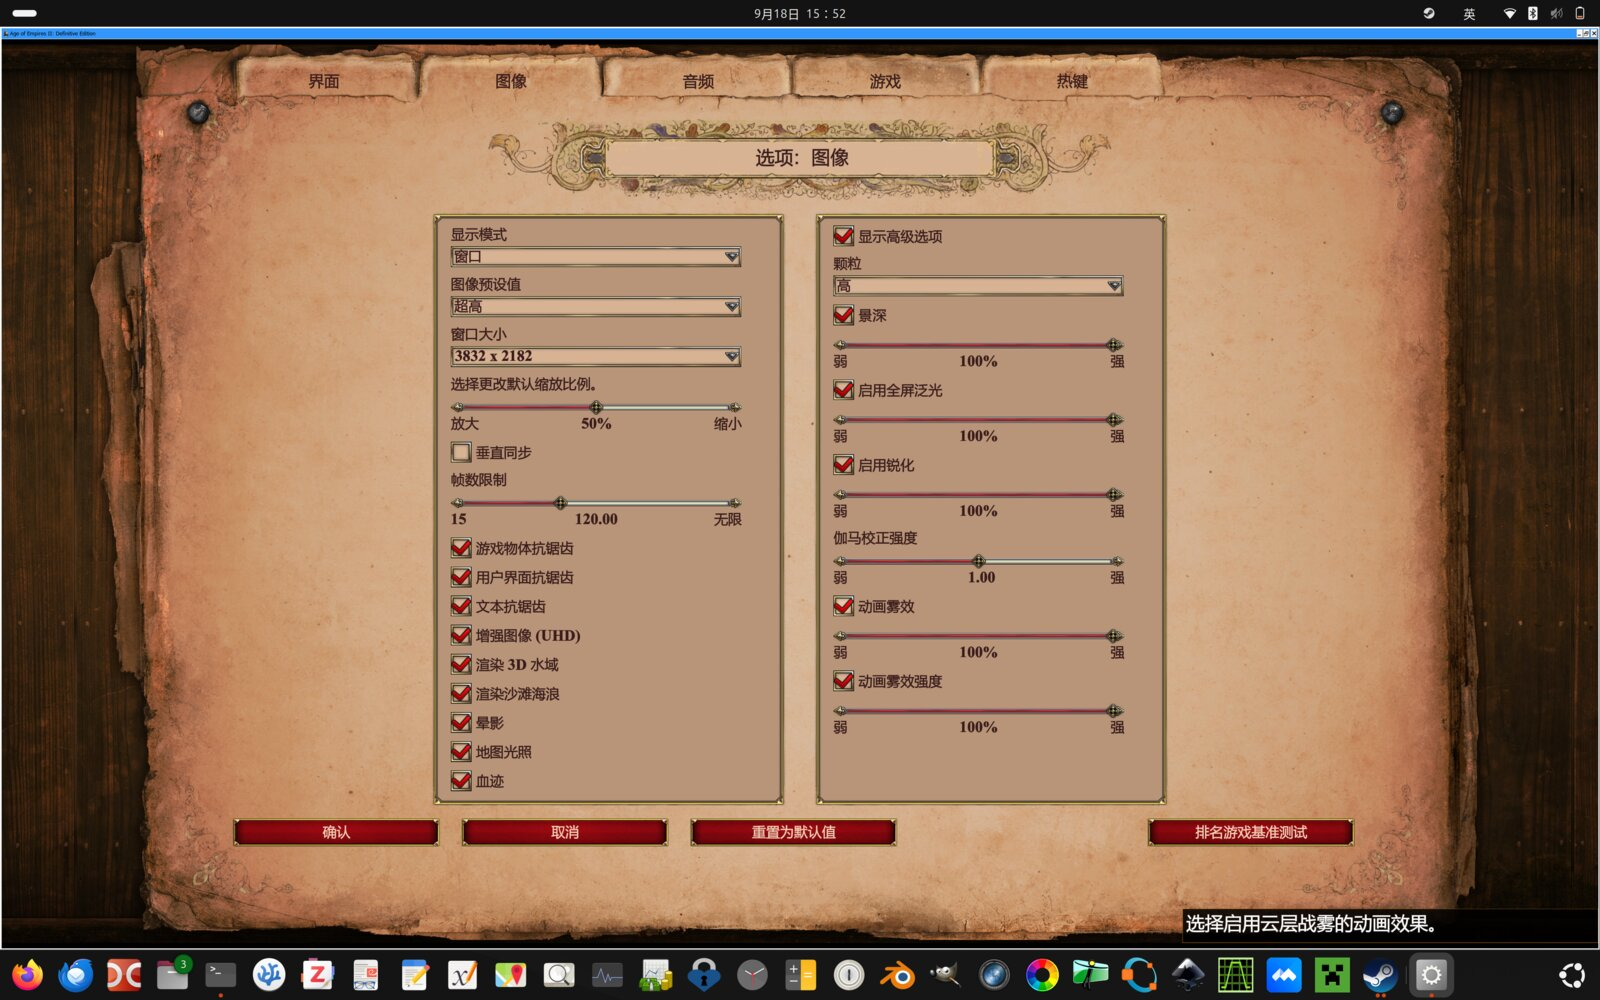
\includegraphics[width=\linewidth]{screen-age-of-empires.jpg}  
            \end{Figure}
        \end{column}
    \end{columns}
\end{frame}

\begin{frame}
    \frametitle{关于显卡}
    \begin{columns}
        \begin{column}{0.53\textwidth}\setlength{\parskip}{6pt}%
            曾几何时，在Linux上使用NVIDIA显卡是一件痛苦的事情，甚至因此诞生了Linus Torvalds非常著名的“FUCK YOU NVIDIA”的演讲名场面。

            但那已经是十多年前的事了。如今NVIDIA的显卡在Linux上都有良好的官方驱动支持，绝大多数情况下，对于游戏和神经网络训练，显卡开箱即用。
        \end{column}
        \begin{column}{0.45\textwidth}
            \begin{Figure}*
                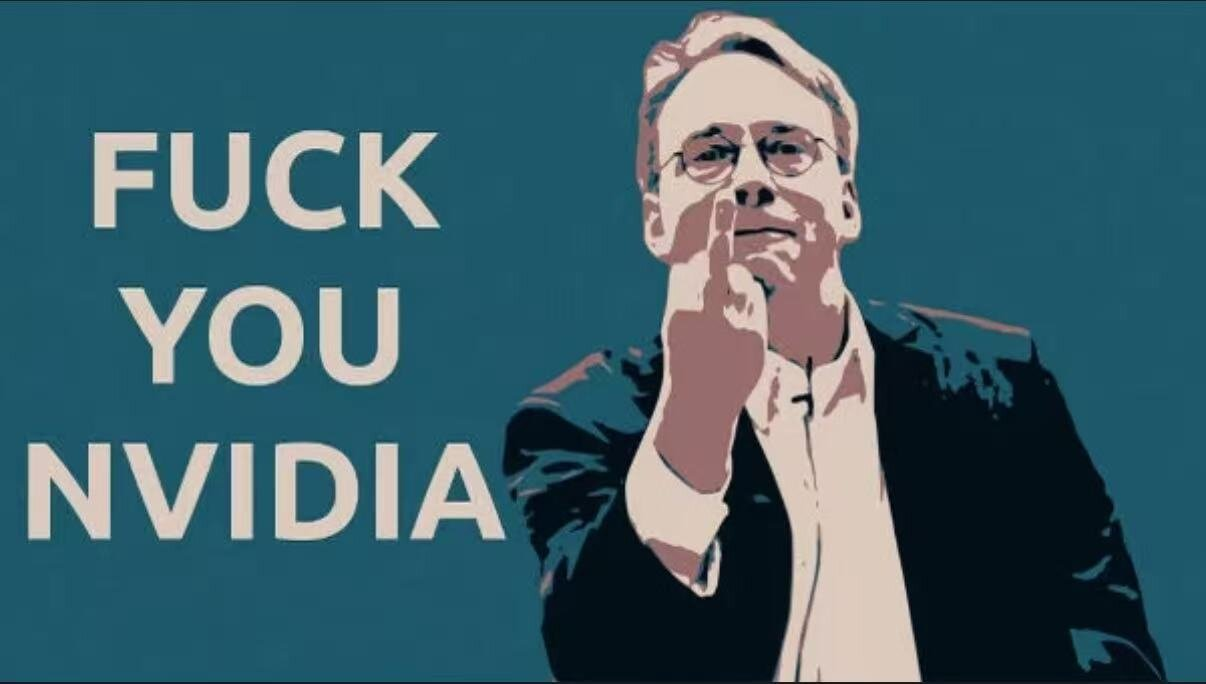
\includegraphics[width=\linewidth]{fuck-u-nvidia.jpg}  
            \end{Figure}
        \end{column}
    \end{columns}
\end{frame}

\begin{frame}
    \frametitle{开始使用Linux}
    本课程提供了两种使用Linux系统的方式
    \begin{itemize}
        \item \alert{WSL}（Windows Subsystem for Linux）：适用于Windows的Linux子系统，是微软官方提供的功能，本质上可以认为是一个在Windows上运行但\alert{只有命令行环境的Linux虚拟机}。该方案适用于想继续使用Windows作为主力系统，只是想获得一个Linux开发环境的学生。
        \item \alert{双系统}：你可以在磁盘上划出一块空间，在保留当前Windows系统的情况下，安装完整的Linux系统。开机时可以选择启动哪个系统。该方案适合希望体验Linux桌面环境的学生。
        \item 推荐使用Ubuntu 26.04或Ubuntu 24.04，但你也可以使用其他Linux发行版。
        \item 此外，对于MacOS用户，你可以直接在MacOS上进行开发，无需Linux虚拟机！
    \end{itemize}
    我们真诚鼓励所有学生尝试双系统方案\footnote{HEAD TA承诺为在安装双系统的过程中遇到技术问题的学生提供技术支持。}，体验在一个完整的Linux桌面系统上工作。
\end{frame}

\begin{frame}
    \frametitle{WSL：最简单的开始方式}
    WSL的安装需要在\alert{正确的网络环境}下，在PowerShell上执行
    \begin{Code}*
        \lstinputlisting[firstline=1,lastline=1]{code/intro/wsl.sh}
    \end{Code}
    WSL在安装后（可能需要重启一次）可以通过以下命令启动
    \begin{Code}*
        \lstinputlisting[firstline=2,lastline=2]{code/intro/wsl.sh}
    \end{Code}
\end{frame}

\begin{frame}
    \frametitle{WSL：最简单的开始方式}
    \begin{itemize}
        \item WSL只有命令行环境，但这不意味着你需要在命令行上编写代码。推荐在Windows上安装VSCode作为代码编辑器，VSCode可以通过“连接到WSL”访问WSL上的文件。
        \item VSCode下载链接：\url{https://code.visualstudio.com/Download}
    \end{itemize}
\end{frame}

\begin{frame}
    \frametitle{双系统：更好的选择}
    \begin{itemize}
        \item 下载Ubuntu 24.04或26.04的系统镜像（ISO）。
        \item 使用BalenaEtcher或Rufus将镜像写入U盘，制作启动盘。
        \item 若Windows启用了BitLocker，\alert{请务必先关闭，否则可能导致Windows损坏}。
        \item 在Windows的磁盘管理中压缩卷，留出未分配空间用于安装Ubuntu。
        \item \url{https://ubuntu.com/download/desktop?version=24.04}
        \item \url{https://ubuntu.com/download/desktop?version=26.04}
        \item \url{https://etcher.balena.io/}
        \item \url{https://rufus.ie/en/}
    \end{itemize}
\end{frame}

\begin{frame}
    \frametitle{双系统：更好的选择}
    \begin{itemize}
        \item 将启动盘插入电脑，重启，按F2、F10或DEL进入BIOS，选择从U盘启动。
        \item 在图形界面中完成安装，注意选择中文语言和第三方驱动。
        \item 在分区配置中选择手动分区，在未分配空间上创建分区并挂载至\code{/}。
        \item 文件系统推荐Btrfs而非默认的Ext4。
        \item \alert{创建分区会格式化对应区域，请务必不要格式化Windows正在使用的分区！}
        \item 在Linux上我们更推荐使用VSCode的开源构建版本VSCodium。
        \item \url{https://vscodium.com/}
    \end{itemize}
\end{frame}

\begin{frame}
    \frametitle{C语言的最小工作示例}
    首先，安装C/C++开发环境（\code{build-essential}打包了\code{gcc}、\code{g++}、\code{make}等工具）
    \begin{Code}*
        \lstinputlisting{code/intro/build-essential.sh}
    \end{Code}
    随后，创建一个\code{main.c}的文件，写入以下内容
    \begin{Code}*{c}
        \lstinputlisting{code/intro/main.c}
    \end{Code}
\end{frame}

\begin{frame}
    \frametitle{C语言的最小工作示例}
    通过以下命令将\code{main.c}编译为执行程序\code{MyProgram}（Linux的执行程序没有后缀）
    \begin{Code}*
        \lstinputlisting{code/intro/gcc-simple.sh}
    \end{Code}
    通过以下命令运行\code{MyProgram} 
    \begin{Code}*
        \lstinputlisting{code/intro/run-program.sh}
    \end{Code}
\end{frame}

\section{Linux的基本命令}

\begin{frame}
    \frametitle{软件包管理器}
    在Linux系统中，几乎所有发行版都采用了某种软件包管理器，例如，Ubuntu的软件包管理器就是\code{apt}，你可以使用\code{apt}命令完成大部分软件的搜索、下载、安装、更新、卸载！
\end{frame}

\begin{frame}
    \frametitle{命令\code{apt}}
    通过\code{apt}可以进行更新，更新会分为两步
    \begin{Code}*
        \lstinputlisting[firstline=1,lastline=2]{code/shell/apt.sh}
    \end{Code}
    其中，\code{update}的作用是刷新软件包索引，以了解有哪些软件可以更新，\code{upgrade}的作用是真正更新软件包，\code{sudo}的含义是以\code{root}身份（Linux下的超级用户）运行。在Linux系统中，系统软件和应用软件是一体的。在安装完系统后，应当立即运行一次上述两条命令进行系统更新。

    使用\code{sudo}需输入密码。在Linux下输入密码是没有回显的，盲输按回车即可。
\end{frame}

\begin{frame}
    \frametitle{命令\code{apt}}
    通过\code{apt}可以安装软件，例如以下命令会安装\code{vim}，这是一个命令行上的编辑器
    \begin{Code}*
        \lstinputlisting[firstline=3,lastline=3]{code/shell/apt.sh}
    \end{Code}
    你不需要指定安装路径！这在Linux系统下有一套严格的规范。
\end{frame}

\begin{frame}
    \frametitle{命令\code{pwd}}
    \code{pwd}用于显示当前路径（Print Working Directory）
    \begin{Code}*
        \lstinputlisting{code/shell/pwd.sh}
    \end{Code}
    你可能会得到类似于\code{/home/liyuxuan}的结果。事实上，当前路径总是会显示在你的命令提示符上，只不过当前用户的家目录会用\texttt{\textasciitilde{}}省略表示。终端启动时，通常默认位于家目录。
\end{frame}

\begin{frame}
    \frametitle{命令\code{ls}}
    \code{ls}用于显示当前路径下的文件（List Directory Contents）
    \begin{Code}*
        \lstinputlisting[firstline=1,lastline=1]{code/shell/ls.sh}
    \end{Code}
    搭配\code{-l}显示详细信息，搭配\code{-a}显示隐藏文件，也可以查看指定路径的文件
    \begin{Code}*
        \lstinputlisting[firstline=2,lastline=4]{code/shell/ls.sh}
    \end{Code}
    Linux命令中，参数以空格分隔，选项以\code{-}或\code{--}开头（短选项/长选项）。
\end{frame}

\begin{frame}
    \frametitle{命令\code{cd}}
    \code{cd}用于移动当前路径（Change Directory）
    \begin{Code}*
        \lstinputlisting[firstline=1,lastline=1]{code/shell/cd.sh}
    \end{Code}
    回到家目录，你可以尝试不同的路径表示方法
    \begin{Code}*
        \lstinputlisting[firstline=2,lastline=3]{code/shell/cd.sh}
    \end{Code}
    Linux中，若路径以根目录\code{/}开头，那就是绝对路径，否则是相对路径。
\end{frame}

\begin{frame}
    \frametitle{命令\code{cd}}
    有两个特殊的目录：用\code{.}代表当前目录，用\code{..}代表上一级目录
    \begin{Code}*
        \lstinputlisting[firstline=4,lastline=5]{code/shell/cd.sh}
    \end{Code}
    Linux中，所有以\code{.}开头的文件都是隐藏文件，用\code{ls -a}查看。
\end{frame}

\begin{frame}
    \frametitle{命令\code{touch}}
    \code{touch}用于刷新时间戳，但如果目标文件不存在，它会创建一个空文件
    \begin{Code}*
        \lstinputlisting[firstline=1,lastline=1]{code/shell/touch.sh}
    \end{Code}
    你可以用\code{ls -l}查看文件的时间戳（即最后修改时间）。
\end{frame}

\begin{frame}
    \frametitle{命令\code{mkdir}}
    \code{mkdir}用于创建目录（Make Directory）
    \begin{Code}*
        \lstinputlisting[firstline=1,lastline=1]{code/shell/mkdir.sh}
    \end{Code}
    你可以在\code{ls -l}中观察第一列，若以\code{d}开头则为目录，若以\code{-}开头则为普通文件。
\end{frame}

\begin{frame}
    \frametitle{命令\code{echo}}
    \code{echo}用于打印文字，请注意任何包含空格的参数需要用双引号包裹
    \begin{Code}*
        \lstinputlisting[firstline=1,lastline=1]{code/shell/echo.sh}
    \end{Code}
    通过\code{>}和\code{>>}可以将命令行上的输出重定向到文件，\code{>}是覆盖，\code{>>}是追加
    \begin{Code}*
        \lstinputlisting[firstline=2,lastline=3]{code/shell/echo.sh}
    \end{Code}
\end{frame}

\begin{frame}
    \frametitle{命令\code{cat}}
    \code{cat}用于查看文件内容（Concatenate）
    \begin{Code}*
        \lstinputlisting[firstline=1,lastline=1]{code/shell/cat.sh}
    \end{Code}
    该命令实际上是Concatenate的缩写，但不妨理解为一只猫挠了一下文件（\^{}\_\^{}）。
\end{frame}

\begin{frame}
    \frametitle{命令\code{vim}}
    \code{vim}是一个命令行上的代码编辑器（你可以用它来编辑任何文本文件！）
    \begin{Code}*
        \lstinputlisting[firstline=1,lastline=1]{code/shell/vim.sh}
    \end{Code}
    Vim有一套非常高效的快捷键体系，但它的使用方式常常会让新手感到困惑，牢记以下几点可以让你至少把它当成一个普通编辑器来使用。Vim启动默认处于普通模式，键盘上几乎每个按键都是快捷键！你会发现你无法编辑文件，正确的做法是按下\code{I}，这会让你进入插入模式，这就和普通编辑器一致了。完成后，你需要按\code{ESC}回到普通模式，输入\code{:wq}进行保存和退出\footnote{关于Vim一个经久不衰的笑话是：如何退出Vim？}。

    Vim常用于编辑需要\code{root}权限的配置文件：这种情况下你无法使用VSCode或VSCodium！
\end{frame}

\begin{frame}
    \frametitle{命令\code{mv}}
    \code{mv}用于重命名或移动文件（Move File）
    \begin{Code}*
        \lstinputlisting[firstline=1,lastline=3]{code/shell/mv.sh}
    \end{Code}
    \begin{itemize}
        \item 若目标是一个已经存在的目录，文件会被移动到该目录下。
        \item 若目标不存在或不是目录，文件会被重命名并移动至目标指定的路径。
    \end{itemize}
    \code{mv}不区分操作对象是文件还是目录，也可以用来重命名或移动目录。
\end{frame}

\begin{frame}
    \frametitle{命令\code{cp}}
    \code{cp}用于复制文件（Copy File）
    \begin{Code}*
        \lstinputlisting[firstline=1,lastline=3]{code/shell/cp.sh}
    \end{Code}
    搭配\code{-r}选项可以递归复制目录
    \begin{Code}*
        \lstinputlisting[firstline=4,lastline=4]{code/shell/cp.sh}
    \end{Code}
\end{frame}

\begin{frame}
    \frametitle{命令\code{rm}}
    \code{rm}用于删除文件（Remove File）
    \begin{Code}*
        \lstinputlisting[firstline=1,lastline=1]{code/shell/rm.sh}
    \end{Code}
    搭配\code{-r}选项可以删除目录
    \begin{Code}*
        \lstinputlisting[firstline=2,lastline=2]{code/shell/rm.sh}
    \end{Code}
    特别需要强调的是，Linux的删除是没有回收站的，三思而后行！
\end{frame}

\begin{frame}
    \frametitle{按下回车前请三思}
    命令行非常高效且强大，但错误的使用会造成格外严重的后果！
    \begin{itemize}
        \item 我正在操作的文件是我想要操作的吗？
        \item 我是否位于正确的目录？这是在本地还是在服务器？
        \item 我是否真的理解我在做什么？尤其是当这条命令是由AI提供的。
    \end{itemize}
    胆大心细，勇敢地探索和学习，谨慎地实施和执行，\alert{对自己的行为负责}。
\end{frame}

\begin{frame}
    \frametitle{著名的危险命令}
    以下是一条非常著名的危险命令，\alert{绝对不要在任何情况下尝试！}
    \begin{Code}*
        \lstinputlisting[firstline=3,lastline=3]{code/shell/rm.sh}
    \end{Code}
    其中，\code{sudo}用于提权，\code{rm}用于删除，\code{-r}允许递归删除，\code{-f}允许强制删除，这会跳过部分带保护的文件的删除确认，最后，删除对象是\code{/}即根目录，因此这条命令会高效且悄无声息地抹去这台Linux系统上的一切数据，甚至包括操作系统自身（WSL上执行还会抹除Windows）！

    \alert{能力越大，责任越大}，请谨慎对待你手中掌握的权限。
\end{frame}

\begin{frame}
    \frametitle{命令\code{ln}}
    \code{ln}用于创建链接（Link File），选项\code{-s}代表创建的是软链接
    \begin{Code}*
        \lstinputlisting[firstline=1,lastline=1]{code/shell/ln.sh}
    \end{Code}
    软链接的工作方式类似于快捷方式：当访问\code{link}时，其实是在访问\code{dir}目录下的内容，但和快捷方式有所不同的是，你的路径不会发生跳转，你仍然会位于\code{/home/liyuxuan/link}下。

    软链接在\code{ls -l}下会显示为\code{l}类型，代表这是一个链接。
\end{frame}

\begin{frame}
    \frametitle{软链接与硬链接}
    链接分为两种，软链接（由\code{ln -s}创建）和硬链接（由\code{ln}创建）
    \begin{itemize}
        \item 软链接类似于C++语言中的指针（本质上是存储地址的变量）。
        \item 硬链接类似于C++语言中的引用（本质上是一个别名）。
    \end{itemize}
    在文件系统层面，文件名和文件本体（inode）通常是一一对应的。硬链接不创建新的文件，而是令一个文件inode能关联到多个文件名上。换言之，如果将硬链接理解为文件名和inode间的链接关系，那么所有文件其实都是硬链接：有些inode只关联到一个文件名，有些inode会关联到多个文件名。硬链接命令的作用是在inode和文件名之间创建额外的链接。当删除文件时，本质上是在减少inode的链接计数，当inode的链接计数归零时，空间才会真正被释放。
\end{frame}

\begin{frame}
    \frametitle{软链接与硬链接}
    软链接则是完全不同的东西，它是一个独立的文件（有自己的inode），只不过这个特殊的文件存储的内容是一个路径，使得你在访问它的时候实际访问到的是别的地方，由此实现了链接。
    \begin{itemize}
        \item 软链接可以链接目录或文件，硬链接通常只被允许链接文件。
        \item 软链接可以跨文件系统链接，硬链接则不可以（inode对每个文件系统独立）。
        \item 软链接只是一个普通文件，删除软链接无影响，删除源则所有软链接失效。
    \end{itemize}
    最佳实践：除非你很清楚自己要做什么，\alert{总是使用软链接}！
\end{frame}

\begin{frame}
    \frametitle{获取帮助}
    几乎所有的命令都可以通过\code{--help}选项查看帮助
    \begin{Code}*
        \lstinputlisting[firstline=1,lastline=1]{code/shell/man.sh}
    \end{Code}
    除此之外，使用\code{man}可以查看某个命令文档
    \begin{Code}*
        \lstinputlisting[firstline=2,lastline=2]{code/shell/man.sh}
    \end{Code}
\end{frame}

\begin{frame}
    \frametitle{命令补全}
    你不必完整输入命令！下面展示了输入命令时如何通过按Tab来自动补全
    \begin{Code}*
        \lstinputlisting{code/how-to-tab.sh}
    \end{Code}
    简而言之，按Tab可以帮助你补全命令和已经存在的路径。但请理解补全不是魔法，它并不能预知你的想法，例如这里的\code{vsp}肯定无法补全出来，因为这是你将要创建的目录的名称。
\end{frame}

\begin{frame}
    \frametitle{命令历史}
    你不必重复输入已经输入过的命令！按向上键和向下键可以翻阅输入过的历史命令。

    除此之外，使用\code{history}可以查看所有输入过的命令
    \begin{Code}*
        \lstinputlisting[firstline=1,lastline=1]{code/shell/history.sh}
    \end{Code}

    如果你要搜索包含特定内容的历史命令，可以用管道\code{|}连接\code{grep}
    \begin{Code}*
        \lstinputlisting[firstline=2,lastline=2]{code/shell/history.sh}
    \end{Code}

    管道\code{|}用于将一个命令的输出重定向到另一个命令的输入，\code{grep}用于文本匹配。
\end{frame}

\begin{frame}
    \frametitle{命令\code{tar}}
    在Linux中，经常会看到\code{.tar.gz}后缀的压缩包
    \begin{itemize}
        \item \code{.tar}代表归档，即将多个文件打包为单个文件，由\code{tar}命令完成。
        \item \code{.gz}代表压缩，即将单个文件进行压缩，由\code{gzip}命令完成。
    \end{itemize}
    但事实上，通过恰当的选项，可以用\code{tar}命令一步完成\code{.tar.gz}的压缩和解压缩。
\end{frame}

\begin{frame}
    \frametitle{命令\code{tar}}
    \code{tar}用于压缩的命令是
    \begin{Code}*
        \lstinputlisting[firstline=1,lastline=1]{code/shell/tar.sh}
    \end{Code}
    \code{tar}用于解压的命令是
    \begin{Code}*
        \lstinputlisting[firstline=2,lastline=2]{code/shell/tar.sh}
    \end{Code}
    其中，选项\code{-c}代表Create，选项\code{-x}代表Extract，选项\code{-v}代表Verbose，这会列出所有压缩和解压的文件（需要静默输出时可以省略），选项\code{-z}代表使用Gzip格式的压缩算法，选项\code{-f}代表File，即指定操作的归档文件。这些选项中\code{-f}必须放在最后，因为其后要跟随一个参数。
    
    此外，在Linux的命令中，短选项允许连写是一个普遍支持的特性。
\end{frame}
\section{Linux的目录结构}

\begin{frame}
    \frametitle{Linux的目录结构}
    Linux系统的目录结构遵循文件系统层次标准（Filesystem Hierarchy Standard，FHS）。这实际上是几乎所有类Unix系统遵循的规范：你甚至可以在MacOS上找到相似的目录层次结构！
\end{frame}

\begin{frame}
    \begin{Table}[Linux的根目录结构]!
        \begin{tblr}{colspec={X[1]X[2]X[1]X[2]},cell{2-Z}{1,3}={font=\ttfamily}}
            目录&用途&目录&用途\\
            /bin   & 用户执行程序 &
                                        /media & 自动挂载点 \\
            /lib   & 动态与静态库 &
                                        /mnt   & 手动挂载点 \\
            /sbin  & 系统执行程序 &
                                        /boot  & 启动引导 \\
            /home  & 普通用户家目录 &
                                        /dev   & 设备文件 \\
            /root  & 超级用户家目录&
                                        /sys   & 设备属性 \\
            /etc   & 配置文件 &
                                        /proc  & 进程信息 \\
            /var   & 可变文件 &
                                        /run   & 进程数据 \\
            /usr   & 系统资源 &
                                        /tmp   & 临时数据 \\
            /opt   & 可选软件 & 
                                        /srv   & 服务数据 \\
        \end{tblr}
    \end{Table}
\end{frame}

\begin{frame}
    \frametitle{目录\code{/bin /lib /sbin}}
    \code{/bin}目录存放了所有用户可以执行的命令
    \begin{Code}*
        \lstinputlisting[firstline=1,lastline=2]{code/fhs/bin.sh}
    \end{Code}
    \code{/bin}目录也会包含大部分通过\code{apt}安装的程序。对于Linux系统，它不会区分所谓“系统自带的基本命令”和“用户安装的应用程序”，因为它们两者本质上都是可以执行的二进制程序。
\end{frame}

\begin{frame}
    \frametitle{目录\code{/bin /lib /sbin}}
    例如，安装\code{build-essential}包，这包含了C/C++开发的基本工具
    \begin{Code}*
        \lstinputlisting[firstline=4,lastline=4]{code/shell/apt.sh}
    \end{Code}
    你现在就可以在\code{/bin}下找到\code{gcc}和\code{make}等工具了
    \begin{Code}*
        \lstinputlisting[firstline=3,lastline=4]{code/fhs/bin.sh}
    \end{Code}
\end{frame}

\begin{frame}
    \frametitle{目录\code{/bin /lib /sbin}}
    \code{/lib}目录存放了所有动态库和静态库 
    \begin{itemize}
        \item 库的本质是预先编译好的通用二进制片段，它可以和应用程序进行链接。
        \item 动态链接库：运行时链接，后缀为\code{.so}，例如C库\code{libc.so}
        \item 静态链接库：编译时链接，后缀为\code{.a}，例如C库\code{libc.a}
    \end{itemize}
    你可以在\code{/lib/x86_64-linux-gnu}下找到\code{libc.so}和\code{libc.a}
    \begin{Code}*
        \lstinputlisting[firstline=1,lastline=2]{code/fhs/lib.sh}
    \end{Code}
\end{frame}

\begin{frame}
    \frametitle{目录\code{/bin /lib /sbin}}
    通常，动态链接是较为常用的。
    
    当你在C程序中写下\texttt{\#include <stdio.h>}以及\code{printf}并编译时，函数\code{printf}的二进制并不会被链接到你的程序中，真正发生的事情是，当你的程序运行到\code{printf}函数时，系统会找到\code{libc.so}并运行对应的二进制，这就是所谓“运行时链接”的含义。动态链接机制使系统中海量的二进制程序不必重复包含C库的片段，而是可以共享一个C库，从而节约大量空间！

\end{frame}

\begin{frame}
    \frametitle{目录\code{/bin /lib /sbin}}
    
    然而，静态链接在某些情况下也有其意义。
    
    当你的C程序最终是在某个裸机的单片机上运行时，根本没有操作系统进行动态链接，此时就需要在编译阶段静态链接用到的函数。空间上也很划算，只需要带上C库中真正用到的部分！
\end{frame}

\begin{frame}
    \frametitle{目录\code{/bin /lib /sbin}}
    \code{/sbin}目录存放了所有\code{root}才能执行的命令
    \begin{Code}*
        \lstinputlisting{code/fhs/sbin.sh}
    \end{Code}
    这是因为，在多人使用的服务器上，普通用户显然不能随意关机和重启！ 
\end{frame}

\begin{frame}
    \frametitle{目录\code{/home /root}}
    \code{/home}和\code{root}都是用户的家目录
    \begin{itemize}
        \item \code{/home}是普通用户的家目录，每个用户在\code{/home}下有同名的家目录。
        \item 用户\code{liyuxuan}的家目录位于\code{/home/liyuxuan}。
        \item 用户的家目录始终可以用\texttt{\textasciitilde{}}表示（取决于当前登录的用户）。
        \item \code{/root}是超级用户的家目录，这是\code{root}作为超级用户在架构上享有的额外特权：其家目录并非位于通常的\code{/home/root}，而是相应地高挂了一级，直接位于根目录\code{/root}下。
    \end{itemize}
\end{frame}

\begin{frame}
    \frametitle{目录\code{/etc}}
    \code{/etc}下存放配置文件，比较典型的例子是\code{hosts}文件
    \begin{Code}*
        \lstinputlisting{code/fhs/etc.sh}
    \end{Code}
    你可以在这里设置本地的DNS解析，例如
    \begin{Code}*
        \lstinputlisting{code/hosts}
    \end{Code}
\end{frame}

\begin{frame}
    \frametitle{目录\code{/var}}
    \code{/var}下存放可变文件，比较典型的例子是\code{apt}的日志
    \begin{Code}*
        \lstinputlisting{code/fhs/var.sh}
    \end{Code}
    你可以在两个文件中分别看到\code{apt}最近的更新记录和当时的命令行输出内容。
\end{frame}

\begin{frame}
    \frametitle{目录\code{/usr}}
    \code{/usr}的全称是Unix System Resource，请注意其和User无关！

    如果你足够细心，仔细观察了\code{ls -l /}的输出，你会注意到\code{/bin /lib /sbin}实际上分别是指向\code{/usr/bin /usr/lib /usr/sbin}的软链接！这是因为早期的实践中，前者存储系统所需的命令和库，后者存储用户安装的命令和库，但是，随着时代发展，现在主流的Linux发行版都选择将这两个目录用软链接的方式合并在一起，不再区分到底是系统所需还是用户安装。
\end{frame}

\begin{frame}
    \frametitle{目录\code{/opt}}
    \code{/opt}用于安装可选的第三方大型软件，例如
    \begin{itemize}
        \item Wolfram Mathematica
        \item Xilinx Vivado
        \item 腾讯会议
    \end{itemize}
    这些软件不遵守标准的目录结构，因此统一在\code{/opt}下为每个软件分配独立的目录。
\end{frame}

\begin{frame}
    \frametitle{目录\code{/media /mnt}}
    \code{/media}和\code{/mnt}分别是自动挂载点和手动挂载点，例如当插入U盘后
    \begin{Code}*
        \lstinputlisting{code/fhs/media.sh}
    \end{Code}
    假如U盘的名称是\code{udisk}，那么你就会在该位置看到出现了一个名为\code{udisk}的目录，该过程被称为挂载（Mount），这一点和Windows中插入U盘会出现新的盘符的行为是不太一样的。
    
    通常移动存储设备都可以被自动挂载至\code{/media}，极少数情况需要手动挂载至\code{/mnt}。
\end{frame}

\begin{frame}
    \frametitle{目录\code{/boot}}
    \code{/boot}目录包含了操作系统正常启动所必须的文件。事实上，当在安装系统进行分区时，你可能会注意到除了被挂载于\code{/}的主分区，还会自动产生一个被挂载于\code{/boot/efi}的启动分区。
\end{frame}

\begin{frame}
    \frametitle{目录\code{/dev}}
    \code{/dev}用于存放设备文件，例如
    \begin{Code}*
        \lstinputlisting{code/fhs/dev.sh}
    \end{Code}
    第一条命令的输出可能会看到\code{nvme0n1p1}和\code{nvme0n1p2}，这对应了在NVMe上连接的SSD的第一个分区（\code{p1}）和第二个分区（\code{p2}）。第二条命令用于查看磁盘占用，观察该命令的输出可以发现，挂载点\code{/}对应的是\code{/dev/nvme0n1p1}，挂载点\code{/boot/efi}对应的是\code{/dev/nvme0n1p2}。
\end{frame}

\begin{frame}
    \frametitle{目录\code{/dev}}
    在Linux系统中，\alert{一切皆文件}。磁盘设备本身也被视为一个文件，这并不是一个真实存在的文件，而是通过文件读写的方式包装了对磁盘设备的数据写入和读取。而挂载的作用，就是将磁盘设备的直接读写操作，转换为我们在文件系统层面所看到的对文件的创建、修改、删除。

    设备文件在\code{ls -l}下会显示为\code{b}或\code{c}类型，代表这是一个块设备或字符设备。
\end{frame}

\begin{frame}
    \frametitle{目录\code{/sys}}
    \code{/sys}用于配置设备属性，例如
    \begin{Code}*
        \lstinputlisting{code/fhs/sys.sh}
    \end{Code}
    第一条命令将关闭键盘灯，第二条命令将开启键盘灯。
    
    这里\code{tee}最终发挥的作用就是将\code{0}和\code{1}写入\code{brightness}文件（重定向\code{>}在这里会有权限问题）。\code{/sys}下的文件是设备属性的反映，通过对\code{/sys}下文件的读写可以查看和控制设备属性。
\end{frame}

\begin{frame}
    \frametitle{目录\code{/proc}}
    \code{/proc}是进程的映射，例如
    \begin{Code}*
        \lstinputlisting{code/fhs/proc.sh}
    \end{Code}
    第一条命令会看到大量数字命名的目录，例如\code{248 3533 55991}。第二条命令用于查看全部进程。通过对照，我们可以发现，进程号和\code{/proc}下的数字命名的目录是一一对应的！
\end{frame}

\begin{frame}
    \frametitle{目录\code{/run /tmp /srv}}
    \code{/run}用于存放进程的数据，\code{/tmp}用于存放任何临时文件，系统重启后自动清空。 

    \code{/srv}用于存放本机对外提供的服务的数据（适用于服务器）。
\end{frame}

\section{Linux的权限管理}

\begin{frame}
    \frametitle{超级用户}
    Linux系统的超级用户称为\code{root}，通常来说，修改家目录外的文件都需要\code{root}权限，普通用户可以通过\code{sudo}临时提权以\code{root}身份执行命令（\code{sudo}的含义是Superuser Do）
    \begin{Code}*
        \lstinputlisting[firstline=1,lastline=2]{code/shell/sudo.sh}
    \end{Code}
    当使用\code{sudo}时，你会被要求输入自己的密码（接下来一段时间不用再次输入）。
\end{frame}

\begin{frame}
    \frametitle{超级用户}
    Linux系统中，使用\code{su}命令（Superuser）可以切换至\code{root}用户，此时你会被要求输入\code{root}用户的密码。然而，大部分发行版出于安全原因都禁止直接以\code{root}用户登录，未设置\code{root}密码，这种情况下，输入任何密码都会被认为是错误的！但有趣的是，你可以使用下面的命令
    \begin{Code}*
        \lstinputlisting[firstline=3,lastline=3]{code/shell/sudo.sh}
    \end{Code}
    换言之，临时以超级用户身份宣布将自己提升至超级用户，只需要输入自己的密码！
\end{frame}

\begin{frame}
    \frametitle{超级用户}
    当然，这并非意味着任何用户都可以轻松登录\code{root}用户！
    
    因为其实并不是所有用户都有使用\code{sudo}的权限。通常来说，在一台多人使用的服务器中，只有极少数作为管理员的用户才能使用\code{sudo}命令。给予\code{sudo}的权限等同于提供\code{root}用户！
\end{frame}

\begin{frame}
    \frametitle{超级用户}
    在\code{root}下工作是危险的！引入\code{sudo}机制的意义在于，让那些可以使用\code{root}用户的人平常仍然在自己的低权限用户下工作，仅在必要时，显式以\code{sudo}获得临时提权，避免误操作。
\end{frame}

\begin{frame}
    \frametitle{权限管理机制}
    Linux系统有一套完善的权限管理机制，它可以保证多个用户同时使用，但各个用户又无法触碰他人的数据。即便在只有一个用户的个人电脑上，理解权限管理的概念也是很有价值的。
\end{frame}

\begin{frame}
    \frametitle{权限管理机制}
    尝试以下命令
    \begin{Code}*
        \lstinputlisting{code/ls-list-shell.sh}
    \end{Code}
    你应当会看到以下输出
    \begin{Code}*
        \lstinputlisting{code/ls-list-result.txt}
    \end{Code}
\end{frame}

\begin{frame}
    \frametitle{文件所有权}
    Linux中每个文件都有两个所有权的概念：\alert{所有者}（User）、\alert{所属组}（Group）
    \begin{itemize}
        \item 所有者位于\code{ls -l}输出的第三列，该例中所有者为\code{liyuxuan}
        \item 所属组位于\code{ls -l}输出的第四列，该例中所属组为\code{liyuxuan}
    \end{itemize}
    所属组的概念服务于一个文件需要被多个用户共享的情况。不过，每个用户都会对应一个同名且仅包含其自身的主组，例如，这里的组\code{liyuxuan}就只包含了\code{liyuxuan}这一个用户。
    
    默认情况下，创建文件的用户和其主组会自动成为文件的所有者和所属组。
\end{frame}

\begin{frame}
    \frametitle{文件权限}
    Linux中的权限有三类：\alert{可读}（\code{r}）、\alert{可写}（\code{w}）、\alert{可执行}（\code{x}）
    \begin{itemize}
        \item \code{r}：最高位（\code{r=4}），读取文件，列出目录中的文件，“可读”。
        \item \code{w}：中间位（\code{w=2}），修改文件，增删目录中的文件，“可写”。
        \item \code{x}：最低位（\code{x=1}），执行文件，进入目录，“可执行”。
    \end{itemize}
    例如，\code{rwx}代表可读可写可执行（记为\code{7}），\code{r--}代表只读（记为\code{4}）。

    在Linux中，执行文件是通过权限而非后缀区分的！例如脚本\code{test.py}只有在添加执行权限之后才能以\code{./test.py}的方式运行，否则就只能显式调用解释器\code{python test.py}运行。
\end{frame}

\begin{frame}
    \frametitle{文件权限}
    Linux中每个文件对于三种用户角色（所有者、所属组、其他人）都会定义\code{rwx}权限
    \begin{itemize}
        \item \code{rw-rw-r--}，所有者\code{rw-}，所属组\code{rw-}，其他人\code{r--}，记为\code{644}。
        \item \code{rwxrwxr-x}，所有者\code{rwx}，所属组\code{rwx}，其他人\code{r-x}，记为\code{755}。
        \item \code{rwxrwxrwx}，所有者\code{rwx}，所属组\code{rwx}，其他人\code{rwx}，记为\code{777}。
    \end{itemize}
    实际上\code{644}、\code{755}、\code{777}分别是文件、目录、软链接的默认权限。
    
    默认情况下创建的文件，对所有者和所属组是可读可写，对其他人可读。目录一般应当是可以进入的，所以均增加了可执行。软链接的权限没有意义，实际取决于被链接文件的权限。
\end{frame}

\begin{frame}
    \frametitle{文件权限}
    既然默认对其他人是可读的，那每个用户的隐私如何保证？答案在家目录的权限
    \begin{Code}*
        \lstinputlisting{code/ls-home.sh}
    \end{Code}
    注意到家目录\code{liyuxuan}的权限是\code{750}而非默认的\code{755}，这保护了下面的文件！
\end{frame}

\begin{frame}
    \frametitle{工作目录的创建尝试}
    尽管用户应当在自己的家目录\texttt{\textasciitilde{}}即\code{/home/liyuxuan}下工作，但实践中\texttt{\textasciitilde{}}下往往会产生许多杂乱的用户配置文件和用户安装软件。如果有\code{root}权限，也可以选择在额外创建一个和家目录平级的\code{/home/workspace}作为自己专用的工作目录（\code{/home}下创建目录需要\code{root}权限）
    \begin{Code}*
        \lstinputlisting{code/workspace.sh}
    \end{Code}
    接下来要做两件事：将目录的所有权转给自己，将目录的权限设置为\code{750}。
\end{frame}

\begin{frame}
    \frametitle{命令\code{chown}}
    \code{chown}用于修改所有权（Change Ownership），冒号前后分别指定所有者和所属组
    \begin{Code}*
        \lstinputlisting{code/shell/chown.sh}
    \end{Code}
    由于在执行命令前，该目录还属于\code{root}，故需加上\code{sudo}进行提权。
\end{frame}

\begin{frame}
    \frametitle{命令\code{chmod}}
    \code{chmod}用于修改权限（Change Mode），可以直接用数字标识
    \begin{Code}*
        \lstinputlisting[firstline=1,lastline=1]{code/shell/chmod.sh}
    \end{Code}
    \code{chmod}的用法很灵活，例如为\code{test.py}添加执行权限
    \begin{Code}*
        \lstinputlisting[firstline=2,lastline=2]{code/shell/chmod.sh}
    \end{Code}
    谨慎处理权限问题！遇到权限不足时随意设置\code{sudo chmod 777}是不负责任的行为。
\end{frame}





\VSPendframe{谢谢观看}

\end{document}
